%%%%%%%%%%%%%%%%%%%%%%%%%%%%%%%%%
% sept 2013 [Jan]: hoekpuntmethode weggehaald, verwezen naar TW2 voor simplex, foutjes verbeterd
%
% mei 2011 [Jan]: alle figuren in tikz gezet, typfoutjes verbeterd, tabellen vereenvoudigd met booktabs
%
% 2/2/11 [Greetje]: voorbeeld omgezet naar euro's; wat typfouten aangepast
% 
% 20/9/02 [Jan]: te lange titel aangepast.
%
% 10/09/01 door Greetje
%   titels uniform gemaakt
%
% 01/09/01 door Greetje          %
%%%%%%%%%%%%%%%%%%%%%%%%%%%%%%%%%

%\documentclass[11pt,a4paper]{report}
%\usepackage[dutch]{babel}

%\begin{document}

\chapter{Mathematische modellen voor lineaire programmering}
\begin{quote}
    \textit{{\small Hierop volgde een korte stilte, en toen ging de
    Ridder weer voort. `Het bedenken van dingen, dat is mijn grote
    talent. Je had zeker wel in de gaten, de laatste keer dat je me
    overeind hielp, dat ik een beetje in gedachten was?'}}

    \textit{{\small `U was \emph{wel} wat ernstig,' zei Alice.}}

     \textit{{\small `Nou, net op dat moment was ik een nieuwe manier
     aan het bedenken om over een hek te komen -- wil je het horen?'}}

     \textit{{\small `Ja, heel graag,' zei Alice beleefd.}}

     \textit{{\small `Ik zal je zeggen hoe ik erop kwam,' zei de Ridder. `Ik zei
     namelijk bij mezelf: ''De enige moeilijkheid zit in de voeten:
     het \emph{hoofd} is al hoog genoeg.'' Welnu, eerst leg ik mijn hoofd
     boven op het hek -- dan is het hoofd hoog genoeg -- dan ga ik op
     mijn hoofd staan -- dan zijn de voeten hoog genoeg, snap je --
     dan ben ik er overheen, snap je'}}

          Uit `Achter de spiegel' -- Lewis Carroll
\end{quote}


\newpage
\section{Voorbeeld 1: Winstmaximalisatie}\label{sec.maxprob}
\subsection{Probleemstelling}
\begin{quote}
Een gepensioneerde boer kweekt kippen en schapen. Wie een uitkering
(bvb.\ pensioen) krijgt mag niet meer dan 16 dieren kweken. De
boerin wil niet meer dan 10 kippen. Het grootbrengen van een
kip kost \euros 10. Voor een schaap is dit \euros 50. De boer beschikt
in totaal over \euros 600. Elke kip levert voor \euros 25 winst
(eieren); elk schaap voor \euros 75 (vlees en wol). Hoeveel kippen
en hoeveel schapen moet de boer kweken om zijn winst zo groot
mogelijk te maken?
\end{quote}

\subsection{Wiskundig model}

Het hierboven geschetste probleem gaan we nu oplossen.
Een na\"{\i}eve oplossingsmethode bestaat erin herhaaldelijk getallen
te zoeken die voldoen aan alle voorwaarden en ze in te vullen
in de opgave tot je een maximum (of minimum) gevonden hebt (\textit{trial
and error}). Voor dit vraagstuk is dit waarschijnlijk zelfs de
snelste methode! Ze gaat bvb.\ als volgt: Je weet dat er maximaal
16 dieren zijn, waarvan ten hoogste 10 kippen. Het ligt hier
voor de hand om met gehele getallen te werken (8,3 kippen lijkt
niet echt zinvol!). Neem bvb.\ 16 schapen en 0 kippen. Het kweken
van 16 schapen kost volgens de gegevens \euros 800. (16 keer 50).
Aangezien de boer slechts \euros 600 ter beschikking heeft, is
dit geen geldige combinatie van dieren. Een volgende mogelijkheid
zou kunnen zijn: 15 schapen en 1 kip. Ook deze combinatie is
te duur. Ga zelf eens het rijtje af, en bereken bij elke zinvolle
combinatie wat de winst voor de boer zal zijn.


Deze trial and error-methode werkt voor heel eenvoudige problemen.
Je kan je echter wel voorstellen dat naarmate het aantal mogelijkheden
toeneemt, de kans om de optimale te vinden sterk zal afnemen.
Denk aan een uitgebreide versie van het beginprobleem: een professionele
boer met maximaal 2000 stuks, die over een budget van enkele
miljoenen beschikt. We voelen hier duidelijk de behoefte de zaken
wat systematischer aan te pakken.

De eerste stap naar een oplossing is een vertaling van de Nederlandse
zinnen uit de opgave naar wiskunde. We bouwen m.a.w. een \textit{wiskundig
model} op. Alle gegevens eens rangschikken in een tabel is
vaak\footnote{Niet elke opgave is hiervoor geschikt, maar als het kan
is het een goede manier om de gegevens uit de opgave wat te
systematiseren.}
een goed vertrekpunt. Wat we uiteindelijk wensen te bepalen zijn
het aantal kippen en het aantal schapen. Deze \textit{onbekenden}
moeten een naam krijgen, bvb.\ $x$ (het aantal kippen) en $y$
(het aantal schapen). Natuurlijk staat het je vrij andere letters
te kiezen (bvb.\ $x_{1}$ en $x_{2}$).

De informatie uit de opgave vatten we samen in tabel~\ref{tbl:opg1}.
\begin{table}[htbp]
    \centering
    \caption{Samenvatting van de opgave}
    \begin{tabular}{lcccc}
        \toprule
         & & kost per dier & winst per dier & maximum \\
        \midrule
        aantal kippen & $x$ & 10 & 25 & 10  \\
        aantal schapen & $y$ & 50 & 75 &  \\
        \cmidrule{2-3}
        maximum & 16  & 600 & &  \\
    \bottomrule
    \end{tabular}
    \label{tbl:opg1}
\end{table}

We maken hiervan gebruik om volgende \textit{beperkingen} op te
schrijven:

\begin{itemize}
    \item  Er zijn $x$ kippen en $y$ schapen. Het totaal aantal dieren dat op de boerderij rondloopt is dus gelijk aan $x+y$. Het totaal aantal dieren mag niet groter zijn dan 16. Dit geeft de beperking  $x+y\leqslant 16$.

    \item  Niet meer dan 10 kippen geeft de beperking  $x\leqslant 10$.

    \item  Het kost \euros 10 om een kip te kweken, \euros 50 voor een
schaap. De totale kost voor het kweken van $x$ kippen en $y$ schapen  is gelijk aan 
$10\cdot x+50\cdot y$.  Aangezien de boer slechts beschikt over \euros 600, moet dit bedrag kleiner zijn dan 600. Dit  leidt tot de beperking $10\cdot x+50\cdot y\leqslant 600$.

    \item  Het aantal kippen en schapen kan niet negatief worden: $x
    \geqslant 0$ en $y \geqslant 0$.
\end{itemize}

De boer wil weten hoeveel kippen en hoeveel schapen hij moet
kweken om zijn winst zo groot mogelijk te maken. Een kip levert
\euros 25 op, een schaap \euros 75. Er zijn $x$ kippen en $y$ schapen zodat de \textit{winstfunctie}
(waarbij $W$ staat
voor winst in \euros) $W = 25\cdot x + 75\cdot y$.
Voor dit vraagstuk komt het er op aan om deze $W$ zo groot
mogelijk te maken.

Samengevat geeft deze opgave aanleiding tot dit wiskundig
model:
\noindent
Maximaliseer
\begin{equation}
    W=25\cdot x + 75\cdot y
    \label{eq:doelf}
\end{equation}
met als beperkingen
\begin{eqnarray}
    x+y & \leqslant & 16
    \label{eq:maxdieren}  \\
    x & \leqslant & 10
    \label{eq:maxkippen}  \\
    10\cdot x+50\cdot y& \leqslant & 600
    \label{eq:maxgeld}  \\
    x & \geqslant & 0
    \label{eq:minkippen}  \\
    y & \geqslant & 0
    \label{eq:minschapen}
\end{eqnarray}


Vergelijking (\ref{eq:doelf}) noemen we algemeen de \emph{doelfunctie}\index{doelfunctie}.
Het is een lineaire \emph{ver}gelijking
(= vergelijking van de eerste graad).
Ongelijkheden (\ref{eq:maxdieren}) tot (\ref{eq:minschapen}) zijn de beperkingen.
Het zijn lineaire \emph{on}gelijkheden
(= ongelijkheden van de eerste graad). Ze beperken de oneindig
grote verzameling van alle \emph{mogelijke} combinaties (bvb.\ 205
kippen en 1589 schapen) tot een -- al dan niet begrensde -- verzameling
van \emph{geldige} combinaties. 

Nu het model opgesteld is, komt 
de volgende stap: \emph{bepaal de verzameling van alle geldige
combinaties} van $x$ en $y$. Dit doen we \emph{grafisch}, omdat er
slechts twee onbekenden zijn. Elke mogelijke combinatie stelt een punt
in het vlak voor. We bakenen in het vlak een gebied af waar de punten voldoen aan de beperkingen. Dit doen we door alle gebieden van punten die n\'iet voldoen aan \'e\'en van de beperkingen te arceren. 

\subsection{Verzameling van alle geldige combinaties}

\subsubsection{Beperking (\ref{eq:maxdieren})}


We beginnen met beperking  (\ref{eq:maxdieren}) die iets zegt over het maximale
aantal dieren. We herschrijven deze ongelijkheid tot er staat: $y \leqslant
\ldots$ of $y \geqslant \ldots$. Dit noemen we de \emph{standaardvorm}\index{standaardvorm}
van de ongelijkheid.

Voor deze beperking vind je gemakkelijk: $y \leqslant -x + 16$. De grens tussen de punten $(x,y)$ die voldoen aan
deze ongelijkheid, en de punten die er niet aan voldoen is de
rechte met vergelijking: $y=-x + 16$.
Om deze rechte te tekenen zijn er verschillende mogelijkheden:

\begin{enumerate}
    \item  Elke rechte ligt ondubbelzinnig vast als je twee (van elkaar
verschillende) punten ervan kent. Bepaal dus twee punten van
de rechte $y=-x+16$ door bvb.\ twee keer een verschillende $x$-waarde
in te vullen, en uit te rekenen wat de bijbehorende $y$-waarde
is 

\begin{center}
    \begin{tabular}{c|c}
    $x$ & $y$  \\
    \hline
    0 & 16  \\
    10 & 6  \\
\end{tabular}


\end{center}

De rechte gaat dus door de punten $(0,16)$ en $(10,6)$. Je merkt
aan deze twee koppels dat de rechte \emph{daalt}: Als de $x$-waarde
toeneemt (van 0 naar 10), daalt de $y$-waarde (van 16 naar
6). In figuur~\ref{fig:maxdierrechte} wordt deze rechte getekend.

\begin{figure}[htbp]
    \centering
\begin{tikzpicture}[scale=0.4]
\draw[->] (-1,0) -- (18,0) node[right] {$x$};
\draw[->] (0,-1) -- (0,18) node[above] {$y$};
\foreach \x in {2,4,...,16}
	\draw[shift={(\x,0)}] (0pt,2pt) -- (0pt,-2pt) node[below] {\footnotesize $\x$};
\foreach \y in {2,4,...,16}
	\draw[shift={(0,\y)},color=black] (2pt,0pt) -- (-2pt,0pt) node[left] {\footnotesize $\y$};
\draw[thick](-1,17) -- (17,-1) node[sloped,above,near end]{\small $x+y=16$};
\draw[dashed](0,6) -| (10,0);
\node [below left] at (0,0) {\footnotesize 0};
\filldraw [red!80] (10,6) circle (4pt);
\end{tikzpicture}
\caption{Rechte met vgl. $y=-x+16$}
    \label{fig:maxdierrechte}
\end{figure}

    \item  Een tweede manier om de rechte te bepalen uitgaande van het functievoorschrift
maakt gebruik van de richtingsco\"{e}ffici\"{e}nt (rico). Bekijken
we de algemene vergelijking van een rechte: $y=mx+q$.
Als we $x$ gelijkstellen aan 0, vinden we $y=q$. Dit
wil zeggen dat de rechte de $y$-as (die als vgl.\ $x=0$ heeft)
snijdt in het punt $(0,q)$. Ga nu vanuit dit punt \'e\'en eenheid naar
rechts (horizontaal). De rico $m$ is het getal dat aangeeft hoeveel eenheden 
je moet stijgen (of dalen) om op een tweede punt van de rechte
uit te komen. In ons geval: $y=-x+16$. Het snijpunt
met de $y$-as is $(0,16)$. De rico is hier $-1$. Als we vanuit het
punt $(0,16)$ \'e\'en eenheid naar rechts gaan, moeten we $-1$ naar boven
gaan, wat gelijk staat aan 1 naar beneden. Een volgend punt is
dus $(1,15)$. Dit proc\'ed\'e kan je herhalen voor eender welk punt op de rechte. De rechte blijkt te dalen onder een hoek van
$45^{\circ}$.
\end{enumerate}


We hebben nu de rechte $y=-x+16$ getekend. Deze rechte verdeelt het vlak in twee gebieden, \emph{halfvlakken}\index{halfvlak} genaamd. In het ene halfvlak voldoen de combinaties $x$ en $y$ w\'el aan de ongelijkheid $y \leqslant -x + 16$. In het andere halfvlak voldoen de combinaties $x$ en $y$ niet aan die ongelijkheid. 


Een eenvoudige manier om te bepalen in welk van de twee halfvlakken
(dat boven de rechte, of het halfvlak dat eronder ligt) de combinaties $x$ en $y$ voldoen aan  de ongelijkheid, is gewoon het invullen van
een punt. We kiezen een gemakkelijk punt in \'e\'en  van de twee
halfvlakken dat niet op de rechte ligt, bvb.\ de oorsprong $(0,0)$, die in het halfvlak onder
de rechte ligt. Invullen in de ongelijkheid levert: $0 \leq
-0+16$. Dit is natuurlijk een ware uitspraak: 0 is inderdaad
kleiner dan of gelijk aan 16. Je besluit bijgevolg dat dit punt
$(0,0)$ voldoet aan de ongelijkheid. Het is niet moeilijk om in
te zien dat elk punt onder de rechte (of erop!) voldoet\footnote{We
spreken af dat we de halfvlakken die \emph{niet} voldoen aan de beperkingen arceren.}
(Figuur~\ref{fig:ongelijkheid}).

\begin{figure}[htbp]
    \centering
\begin{tikzpicture}[scale=0.4]
\draw[->] (-1,0) -- (18,0) node[right] {$x$};
\draw[->] (0,-1) -- (0,18) node[above] {$y$};
\foreach \x in {2,4,...,16}
	\draw[shift={(\x,0)}] (0pt,2pt) -- (0pt,-2pt) node[below] {\footnotesize $\x$};
\foreach \y in {2,4,...,16}
	\draw[shift={(0,\y)},color=black] (2pt,0pt) -- (-2pt,0pt) node[left] {\footnotesize $\y$};
\node [below left] at (0,0) {\footnotesize 0};	
	\fill[pattern=north east lines, pattern color=gray]  (17,-1) -- (17,17) -- (-1,17) -- cycle;
\draw[thick](-1,17) -- (17,-1) node[sloped,below,near end]{\small $x+y\leqslant 16$};
\end{tikzpicture}
    \caption{Gearceerde punten voldoen niet aan ongelijkheid $y \leqslant -x+16$}
    \label{fig:ongelijkheid}
\end{figure}

Omgekeerd is het ook zo dat je boven de rechte (het gearceerde
gebied) geen enkel geldige oplossing voor de ongelijkheid kunt
vinden. M.a.w.\ alle punten die voldoen aan de gegeven lineaire ongelijkheid
liggen op of onder de rechte met vergelijking $y=-x+16$.



\subsubsection{Beperking (\ref{eq:maxkippen})}
De lineaire ongelijkheid $x \leqslant 10$ kan niet in de standaardvorm
geschreven worden vermits er geen $y$ in de ongelijkheid staat.
De rechte  $x=10$ is inderdaad een buitenbeen:
het is een \emph{verticale rechte} die gaat door de punten (10,
0), (10, 1) (10, -75),\ldots Aangezien bij \'{e}\'{e}n $x$ oneindig
veel verschillende $y$-waarden mogelijk zijn, stelt deze vergelijking
\emph{geen} functie voor. Alle oplossingen van ongelijkheid (\ref{eq:maxkippen}) liggen links van, of op
de verticale rechte (Figuur~\ref{fig:vertrechte}):
\begin{figure}[htbp]
    \centering
\begin{tikzpicture}[scale=0.4]
	\fill[pattern=north east lines, pattern color=gray]  (10,-1) -- (14,-1) -- (14,10) --(10,10) -- cycle;
\draw[->] (-1,0) -- (16,0) node[right] {$x$};
\draw[->] (0,-1) -- (0,10) node[above] {$y$};
\foreach \x in {2,4,...,14}
	\draw[shift={(\x,0)}] (0pt,2pt) -- (0pt,-2pt) node[below] {\footnotesize $\x$};
\foreach \y in {2,4,...,8}
	\draw[shift={(0,\y)},color=black] (2pt,0pt) -- (-2pt,0pt) node[left] {\footnotesize $\y$};
\node [below left] at (0,0) {\footnotesize 0};	

\draw[thick](10,-1) -- (10,10) node[left,very near end]{\small $x\leqslant 10$};
\end{tikzpicture}
    \caption{Grafische voorstelling van beperking (\ref{eq:maxkippen})}
    \label{fig:vertrechte}
\end{figure}



\subsubsection{Beperking (\ref{eq:maxgeld})}
Herschrijf deze ongelijkheid tot de standaardvorm. Je vindt:
\begin{align*}
    10x+50y &\leqslant 600 \\
     & \Updownarrow   \\
    50y & \leqslant  -10x+600  \\
     & \Updownarrow    \\
    y & \leqslant  -\frac{10}{50}x+\frac{600}{50}  \\
     & \Updownarrow    \\
    y & \leqslant  -\frac{1}{5}x+12
\end{align*}
Deze ongelijkheid staat nu in de standaardvorm. Als we $\leqslant$
vervangen door `$=$' wordt de ongelijkheid een lineaire gelijkheid,
dus een rechte. Deze rechte heeft als vgl. $y=-\frac{1}{5}x+12$.
Ze gaat door het punt $(0,12)$ en is dalend (rico $=-\frac{1}{5}$)
Je bekomt het halfvlak uit figuur~\ref{fig:budget} (opnieuw onder, en op de
rechte):
\begin{figure}[tbp]
    \centering
\begin{tikzpicture}[scale=0.4]
\draw[->] (-1,0) -- (20,0) node[right] {$x$};
\draw[->] (0,-1) -- (0,15) node[above] {$y$};
\foreach \x in {2,4,...,18}
	\draw[shift={(\x,0)}] (0pt,2pt) -- (0pt,-2pt) node[below] {\footnotesize $\x$};
\foreach \y in {2,4,...,14}
	\draw[shift={(0,\y)},color=black] (2pt,0pt) -- (-2pt,0pt) node[left] {\footnotesize $\y$};
\node [below left] at (0,0) {\footnotesize 0};	
	\fill[pattern=north east lines, pattern color=gray]  (20,8) -- (20,14) -- (-1,14)-- (-1,12.2) -- cycle;
\draw[thick](-1,12.2) -- (20,8) node[sloped,below,near end]{\small $10x+50y\leqslant 600$};
\draw[dashed](0,10) -| (10,0);
\filldraw [red!80] (10,10) circle (4pt);
\end{tikzpicture}
    \caption{Beperking $10x+50y 
    \leqslant 600$}
    \label{fig:budget}
\end{figure}



\subsubsection{Beperkingen (\ref{eq:minkippen}) en (\ref{eq:minschapen})}
Deze twee beperkingen zijn heel gelijkaardig: allebei zeggen
ze dat je voor deze opgave geen negatieve getallen ($-3$ schapen
en $-7$ kippen!) kan krijgen. De ongelijkheid $x \geqslant 0$ komt overeen met het halfvlak rechts van de
$y$-as; $y \geqslant 0$ is het halfvlak boven de $x$-as
(figuur~\ref{fig:eenkwadrant}).
\begin{figure}[htbp]
    \centering
\begin{tikzpicture}[scale=1]
\draw[->] (-0.8,0) -- (4.2,0) node[right] {$x$};
\draw[->] (0,-0.8) -- (0,4.2) node[above] {$y$};
\node [below left] at (0,0) {\footnotesize 0};	
	\fill[pattern=north east lines, pattern color=gray]  (4,0) -- (4,-1) -- (-1,-1)-- (-1,4) -- (0,4) -- (0,0) -- cycle;
	\node at (2,2) {\small $x\geqslant 0 \text{ en } y\geqslant 0$};
\end{tikzpicture}
    \caption{Enkel punten in het eerste kwadrant voldoen}
    \label{fig:eenkwadrant}
\end{figure}



\subsubsection{Alle beperkingen samen}
Alle punten die aan elk van de vijf beperkingen tegelijkertijd voldoen
behoren tot de verzameling van de geldige combinaties. Je vindt
heel deze verzameling door een doorsnede te maken van alle bovenstaande
grafische oplossingen (half-vlakken). Enkel het gebied dat in
geen van de voorgaande figuren gearceerd was, hou je over als
geldige oplossingenverzameling. Dit gebied blijkt een vijfhoek
-- gelegen in het eerste kwadrant --
te zijn (figuur~\ref{fig:allebep}).
\begin{figure}[htbp]
    \centering
\begin{tikzpicture}[scale=0.4]
\draw[->] (-1,0) -- (20,0) node[right] {$x$};
\draw[->] (0,-1) -- (0,18) node[above] {$y$};
\foreach \x in {2,4,...,18}
	\draw[shift={(\x,0)}] (0pt,2pt) -- (0pt,-2pt) node[below] {\footnotesize $\x$};
\foreach \y in {2,4,...,16}
	\draw[shift={(0,\y)},color=black] (2pt,0pt) -- (-2pt,0pt) node[left] {\footnotesize $\y$};
\node [below left] at (0,0) {\footnotesize 0};	
	\fill[pattern=north east lines, pattern color=gray]  (-1,12.2) -- (5,11)-- (10,6) -- (10,-1) -- (18,-1) -- (18,17) -- (-1,17) -- cycle;
\draw[thick](-1,12.2) -- (20,8);
\draw[thick](10,-1) -- (10,16);
\draw[thick](-1,17) -- (17,-1);
\draw[very thick, red] (0,0) -- (10,0) -- (10,6) -- (5,11) -- (0,12) -- cycle;
\end{tikzpicture}
    \caption{Alle beperkingen samen: geldige oplossingenverzameling}
    \label{fig:allebep}
\end{figure}



\subsection{De doelfunctie}
Vergelijking (\ref{eq:doelf}) is de doelfunctie. We zoeken die combinatie
van $x$ en $y$ die de winst $W$ zo groot mogelijk maakt.
Vanzelfsprekend moeten we ons beperken tot alle \emph{geldige} combinaties $x$
en $y$.

De doelfunctie is een lineaire
vergelijking van de eerste graad. Alle punten $(x, y)$
die er aan voldoen liggen op een rechte. Deze rechte krijgt de
naam \emph{isowinstrechte} (``rechte van gelijke (= `iso') winst''):
het is de verzameling van al die punten $(x, y)$ die eenzelfde
winst $W$ opleveren. We herschrijven de doelfunctie tot de
standaardvorm:
\begin{align*}
    W &=  25x+75y  \\
     & \Updownarrow    \\
    75y &=  -25x+W  \\
     & \Updownarrow    \\
    y &=  -\frac{25}{75}x+\frac{W}{75}  \\
     & \Updownarrow    \\
    y &=  -\frac{1}{3}x+\frac{W}{75}
\end{align*}
Deze rechte heeft als rico $-\frac{1}{3}$ en snijdt de $y$-as in het punt
$(0,\frac{W}{75})$. Dit snijpunt hangt dus af van de waarde $W$.
We zoeken nu voor dit vraagstuk een realistische waarde voor
$W$. Een goed vertrekpunt is bvb.\ een punt uit de geldige oplossingenverzameling
te nemen en in te vullen in de winstfunctie. We nemen 	
bij voorkeur een gemakkelijk punt, bvb.\ $(10, 0)$. Tien kippen
en 0 schapen voldoet inderdaad aan alle voorwaarden. Dit punt
levert een winst op van $25\cdot 10 + 75\cdot 0 = 250$.
Dit getal blijkt een realistisch
winstcijfer te zijn. Geven we $W$ achtereenvolgens de waarde
250,  300, 450, dan krijgen we de rechten
uit figuur~\ref{fig:isowinstrechten}
\begin{figure}[htbp]
    \centering
\begin{tikzpicture}[scale=0.4]
\draw[->] (-1,0) -- (21.4,0) node[right] {$x$};
\draw[->] (0,-1) -- (0,9) node[above] {$y$};
\foreach \x in {2,4,...,20}
	\draw[shift={(\x,0)}] (0pt,2pt) -- (0pt,-2pt) node[below] {\footnotesize $\x$};
\foreach \y in {2,4,...,8}
	\draw[shift={(0,\y)},color=black] (2pt,0pt) -- (-2pt,0pt) node[left] {\footnotesize $\y$};
\node [below left] at (0,0) {\footnotesize 0};	
\draw[thick,donkergroen](-1,3.667) -- (13,-1) node[sloped,below,midway]{\small $W=250$};
\draw[thick,donkergroen](-1,4.33) -- (15,-1) node[sloped,above,near end]{\small $W=300$};
\draw[thick,donkergroen](-1,6.33) -- (21,-1) node[sloped,above,near end]{\small $W=450$};
\end{tikzpicture}
    \caption{Isowinstrechten voor $W$ = 250, 300 en 450}
    \label{fig:isowinstrechten}
\end{figure}

Aangezien de rico voor de vier rechten \emph{gelijk} is, lopen ze \emph{evenwijdig}.
De rico is tevens een negatief getal, dus zijn het \emph{dalende}
rechten. Naarmate de $W$ die we kiezen groter wordt, schuift
de rechte naar boven. Als $W= 250$, snijdt de rechte de
$y$-as in het punt $(0, \frac{250}{75}=3,333)$. Voor $W= 300$ wordt dit $(0; 4)$,
enz\ldots




\subsection{Grafische oplossing}
We brengen nu de tekening van de geldige combinaties (de gearceerde
veelhoek van figuur~\ref{fig:allebep}) samen met bovenstaande tekening van de isowinstrechten (figuur~\ref{fig:isowinstrechten}). Dit geeft figuur~\ref{fig:allessamengroot}. Omwille van de duidelijkheid pasten
we de schaal aan.
\begin{figure}[htbp]
    \centering
\begin{tikzpicture}[scale=0.6]
\draw[->] (-1,0) -- (17,0) node[right] {$x$};
\draw[->] (0,-1) -- (0,17) node[above] {$y$};
\foreach \x in {2,4,...,16}
	\draw[shift={(\x,0)}] (0pt,2pt) -- (0pt,-2pt) node[below] {\footnotesize $\x$};
\foreach \y in {2,4,...,16}
	\draw[shift={(0,\y)},color=black] (2pt,0pt) -- (-2pt,0pt) node[left] {\footnotesize $\y$};
\node [below left] at (0,0) {\footnotesize 0};	
%	\fill[pattern=north east lines, pattern color=gray]  (-1,12.2) -- (5,11)-- (10,6) -- (10,-1) -- (18,-1) -- (18,17) -- (-1,17) -- cycle;
\draw[](-1,12.2) -- (14,9.2);
\draw[](10,-1) -- (10,12);
\draw[](-1,17) -- (17,-1);
\draw[very thick, red] (0,0) -- (10,0) -- (10,6) -- (5,11) -- (0,12) -- cycle;
\draw[thick,donkergroen](-1,7) -- (16,1.333) node[sloped,above,near end]{\small $W=500$};
\draw[dashed](0,5) -| (5,0);
\filldraw [donkergroen] (5,5) circle (4pt);
\node (A) [above] at (5,5) {A};
\draw[thick,donkergroen](0,9.333) -- (16,4) node[sloped,above,near end]{\small $W=700$};
\draw[dashed](0,8) -| (4,0);
\filldraw [donkergroen] (4,8) circle (4pt);
\node (B) [above] at (4,8) {B};
\draw[thick,donkergroen](0,12) -- (16,6.67) node[sloped,above,near end]{\small $W=900$};
\draw[dashed](0,11) -| (3,0);
\filldraw [donkergroen] (3,11) circle (4pt);
\node (C) [above] at (3,11) {C};
\draw[dashed](0,10) -| (6,0);
\filldraw [donkergroen] (6,10) circle (4pt);
\node (D) [above] at (6,10) {D};
\end{tikzpicture}
    \caption{Overzichtstekening voor voorbeeld 1}
    \label{fig:allessamengroot}
\end{figure}

Stel: de boer
kweekt 5 kippen   en 5 schapen. Deze situatie komt in het vlak overeen met het punt $A(5,5)$. De winst die
de boer daarmee maakt is  $W = 25\cdot 5 + 75\cdot 5 = 500$.
Dit punt ligt zoals je kan zien op figuur~\ref{fig:allessamengroot} op de isowinstrechte
van 500. Bekijk het punt $B(4, 8)$ in deze
figuur.
Het is een geldige combinatie
want dit punt ligt in de veelhoek. 4 kippen en 8 schapen leveren
een winst op van $W = 25\cdot 4 + 75\cdot 8 = 700$.
Het punt $(4, 8)$ ligt bijgevolg op de isowinstrechte waarvoor $W=700$.\\
Er zijn echter combinaties die voor de boer nog hogere winst
opleveren. De isowinstrechte waarvoor $W= 900$ loopt nog
een klein stukje door de geldige oplossingenverzameling.

Het punt $C(3,11)$ behoort  tot de geldige oplossingenverzameling.
Het is een punt van de isowinstrechte waarvoor $W= 900$ ($ 25\cdot
3 + 75\cdot11=900$). Het punt $D(6,10)$ ligt op dezelfde isowinstrechte ($25\cdot 6+75\cdot 10=900$). 
Zijn $(3, 11)$ en $(6, 10)$ nu de optimale combinaties?
Je ziet op figuur~\ref{fig:allessamengroot} dat de isowinstrechte nog naar boven
kan opschuiven binnen de geldige oplossingenverzameling. Probeer zelf met een lat of geo-driehoek
de isowinst evenwijdig met de isowinstlijn van 700 op te
schuiven tot je het gearceerde gebied net binnendringt.
Het is duidelijk dat dit optimale punt een \emph{hoekpunt van de
veelhoek} is.
Dit hoekpunt kan op verschillende manieren berekend worden:

\begin{itemize}
    \item  Je kan het (benaderend) aflezen op de tekening.

    \item  Via een eenvoudig stelsel kan de oplossing gezocht worden als het
snijpunt $E$ van twee rechten. Hier bvb.\ met de substitutie-methode:
\end{itemize}
\begin{eqnarray*}
     &  &
    \left\{\begin{array}{l}
         x+y=16  \\
         10x+50y=600
     \end{array}
     \right.
       \\
     & \Leftrightarrow &  \left\{\begin{array}{l}
         x=16-y  \\
         10(16-y)+50y=600
     \end{array}
     \right. \\
     & \Leftrightarrow & \left\{\begin{array}{l}
         x=16-y  \\
         y=11
     \end{array}
     \right.  \\
     & \Leftrightarrow & \left\{\begin{array}{l}
         x=5  \\
         y=11
     \end{array}
     \right.
\end{eqnarray*}



Je vindt uiteindelijk als co\"{o}rdinaten voor het hoekpunt $(5,
11)$. Door dit punt gaat de isowinstrechte waarvoor $W= 950$ (figuur~\ref{fig:maxwinstrechte}).
\begin{figure}[htbp]
    \centering
\begin{tikzpicture}[scale=0.5]
\draw[->] (-1,0) -- (17,0) node[right] {$x$};
\draw[->] (0,-1) -- (0,17) node[above] {$y$};
\foreach \x in {2,4,...,16}
	\draw[shift={(\x,0)}] (0pt,2pt) -- (0pt,-2pt) node[below] {\footnotesize $\x$};
\foreach \y in {2,4,...,16}
	\draw[shift={(0,\y)},color=black] (2pt,0pt) -- (-2pt,0pt) node[left] {\footnotesize $\y$};
\node [below left] at (0,0) {\footnotesize 0};	
%	\fill[pattern=north east lines, pattern color=gray]  (-1,12.2) -- (5,11)-- (10,6) -- (10,-1) -- (18,-1) -- (18,17) -- (-1,17) -- cycle;
\draw[](-1,12.2) -- (14,9.2);
\draw[](10,-1) -- (10,12);
\draw[](-1,17) -- (17,-1);
\draw[very thick, red] (0,0) -- (10,0) -- (10,6) -- (5,11) -- (0,12) -- cycle;
\draw[very thick,donkergroen](0,12.67) -- (16,7.33) node[sloped,above,near end]{\small $W=950$};
\draw[dashed](0,11) -| (5,0);
\filldraw [donkergroen,very thick] (5,11) circle (4pt);
\node (E) [above] at (5,11) {E};

\end{tikzpicture}
     \caption{Optimale oplossing}
    \label{fig:maxwinstrechte}
\end{figure}




\subsection{Oplossing}
Elke vraag verdient een (volledig) antwoord, dus even alles op
een rijtje: de optimale oplossing voor de boer bestaat erin 5 kippen en 11
schapen groot te brengen. Dit kan nog net binnen de grenzen van
zijn budget. Het totaal aantal dieren is maximaal, maar het aantal kippen is onder de grens.
Het levert hem een winst van \euros{950} op. Uit
bovenstaand verhaal zou het moeten duidelijk zijn dat de boer
onmogelijk meer winst kan halen en toch nog voldoen aan alle
gestelde voorwaarden.





\newpage
\section{Voorbeeld 2: Kostenminimalisatie}\label{sec.minprob}

\begin{quote}
    Els is ziek en moet vitaminepillen nemen. Elke dag heeft ze ten minste
    16 eenheden vitamine A, 5 eenheden vitamine B, en 20 eenheden
    vitamine C nodig. Ze heeft de keuze tussen twee soorten pillen.
    De rode pillen kosten 20 eurocent per stuk en bevatten 8 eenheden
    A, 1 eenheid B en 2 eenheden C. De blauwe pillen kosten 50 eurocent
    per stuk en bevatten 2 eenheden A, 1 eenheid B en 7 eenheden
    C. Hoeveel rode en blauwe pillen moet ze nemen om in haar dagelijkse
    vitaminebehoefte te voorzien \emph{op de goedkoopste manier}.
\end{quote}



\subsection{Opstellen van het model}

We volgen hier dezelfde stappen als bij het eerste voorbeeld.
Men vraagt het aantal rode en het aantal blauwe pillen te zoeken.
Laten we deze aantallen voorstellen door $x$ (aantal rode
pillen per dag) en $y$ (aantal blauwe pillen per dag).
Een schematisch overzicht (tabel~\ref{tbl:minschema})
kan ook hier goede diensten bewijzen:


\begin{table}[hbp]
    \centering
    \caption{Schema gegevens minimumprobleem}
    \begin{tabular}{rccccc}
    \toprule
       & & Vit. A  & Vit. B & Vit. C & Kost per pil  \\
       & & per pil & per pil& per pil&  (eurocent)  \\
    \midrule
    Aantal rode pillen & $x$ & 8 & 1 & 2 & 20  \\
    Aantal blauwe pillen & $y$ & 2 & 1 & 7 & 50  \\
\cmidrule{3-5}
    min. behoefte &  & 16 & 5 & 20 &   \\
    \bottomrule
\end{tabular}
    \label{tbl:minschema}
\end{table}

De doelfunctie (die minimaal moet gemaakt worden) geeft de totale
kost $K$ per dag weer:
\begin{displaymath}
    K=20x + 50y
\end{displaymath}

De beperkingen houden verband met de minimale hoeveelheden van
elke vitamine die Els moet innemen:
\begin{itemize}
    \item  Van vitamine A moeten er elke dag minstens 16 eenheden aanwezig
zijn: $8x + 2y \geqslant 16$.

    \item  Vitamine B: de minimale dosis  bedraagt 5 eenheden: $x+y\geqslant 5$.

    \item  Vitamine C: $2x + 7y \geqslant 20$.

    \item  Het is niet erg logisch dat iemand een negatief aantal pillen
zou nemen. Daarom kunnen we, net als in het eerste voorbeeld,
eisen dat er geen negatieve getallen voorkomen: $x\geqslant 0$
en $y \geqslant 0$.
\end{itemize}



\subsection{Verzameling geldige oplossingen}
We schetsen  de vijf lineaire ongelijkheden  in 
figuur~\ref{fig:minoplverz}. 
\begin{figure}[tbp]
    \centering
\begin{tikzpicture}[scale=0.8]
\draw[->] (-0.5,0) -- (11.5,0) node[right] {$x$};
\draw[->] (0,-0.5) -- (0,9.5) node[above] {$y$};
\foreach \x in {1,...,11}
	\draw[shift={(\x,0)}] (0pt,2pt) -- (0pt,-2pt) node[below] {\footnotesize $\x$};
\foreach \y in {1,...,9}
	\draw[shift={(0,\y)},color=black] (2pt,0pt) -- (-2pt,0pt) node[left] {\footnotesize $\y$};
\node [below left] at (0,0) {\footnotesize 0};	
\draw[thick](-0.5,10) -- (2.125,-0.5) node[sloped,above,near start]{\small $4x+y\geqslant 8$};
\draw[thick](-0.5,5.5) -- (5.5,-0.5) node[sloped,above,midway]{\small $x+y\geqslant 5$};
\draw[thick](-0.5,3) -- (10,-0) node[sloped,above,near end]{\small $2x+7y\geqslant 20$};
\fill[pattern=north east lines, pattern color=gray]  (0,8) -- (1,4)-- (3,2) -- (10,0) -- (0,0) -- cycle;
\draw[<->,very thick, red] (0,9.5) --(0,8) -- (1,4) -- (3,2) -- (10,0) -- (11.5,0);
\end{tikzpicture}
    \caption{Geldige oplossingenverzameling voor het
    minimalisatieprobleem}
    \label{fig:minoplverz}
\end{figure}

Onmiddellijk valt een groot onderscheid op: Bij het `kippen en
schapen'-voorbeeld is de verzameling van alle geldige oplossingen
een gesloten veelhoek. Er is m.a.w. slechts een beperkt aantal
mogelijke combinaties. Bij dit voorbeeld echter zijn er \emph{oneindig
veel mogelijke combinaties}. Waarschijnlijk sterft Els wel van
een overdosis, maar wiskundig gezien voldoet het innemen van
bvb. 12\,000 rode en 50\,000 blauwe pillen aan alle voorwaarden.



\subsection{Doelfunctie (isokostenfunctie)}
Herwerken van de doelfunctie levert:
\begin{displaymath}
    y=-\frac{2}{5}x+\frac{K}{50}
\end{displaymath}
In figuur~\ref{fig:isoK} tekenen we deze functie voor $K=210,~260,~310,~360$. 
\begin{figure}[htbp]
    \centering
\begin{tikzpicture}[scale=0.7]
\draw[->] (-0.5,0) -- (10.5,0) node[right] {$x$};
\draw[->] (0,-1) -- (0,8.5) node[above] {$y$};
\foreach \x in {1,...,10}
	\draw[shift={(\x,0)}] (0pt,2pt) -- (0pt,-2pt) node[below] {\footnotesize $\x$};
\foreach \y in {1,...,8}
	\draw[shift={(0,\y)},color=black] (2pt,0pt) -- (-2pt,0pt) node[left] {\footnotesize $\y$};
\node [below left] at (0,0) {\footnotesize 0};	
\draw[thick,donkergroen](-0.5,4.4) -- (10,0.2) node[sloped,below,midway]{\small $K=210$};
\draw[thick,donkergroen](-0.5,5.4) -- (10,1.2) node[sloped,below,midway]{\small $K=260$};
\draw[thick,donkergroen](-0.5,6.4) -- (10,2.2) node[sloped,below,midway]{\small $K=310$};
\draw[thick,donkergroen](-0.5,7.4) -- (10,3.2) node[sloped,below,midway]{\small $K=360$};
\end{tikzpicture}
    \caption{Isokostenrechten voor $K=210,~260,~310,~360$}
    \label{fig:isoK}
\end{figure}

Opnieuw vinden we een aantal evenwijdige rechten. Alle punten
die op dezelfde rechte liggen zijn combinaties van rode en blauwe
pillen die hetzelfde kosten. Hoe lager de rechte ligt, des te
lager de kost.

Het komt er nu op aan die isokostenrechte te zoeken die nog net
één of meerdere punten gemeen heeft met de verzameling van de geldige
oplossingen. In figuur~\ref{fig:minsamen} combineren we daarom de twee vorige grafieken (figuren \ref{fig:isoK}
en \ref{fig:minoplverz}). 
\begin{figure}[htbp]
    \centering
\begin{tikzpicture}[scale=0.8]
\draw[->] (-0.5,0) -- (11.5,0) node[right] {$x$};
\draw[->] (0,-0.5) -- (0,9.5) node[above] {$y$};
\foreach \x in {1,...,11}
	\draw[shift={(\x,0)}] (0pt,2pt) -- (0pt,-2pt) node[below] {\footnotesize $\x$};
\foreach \y in {1,...,9}
	\draw[shift={(0,\y)},color=black] (2pt,0pt) -- (-2pt,0pt) node[left] {\footnotesize $\y$};
\node [below left] at (0,0) {\footnotesize 0};	
\draw[](-0.5,10) -- (2.125,-0.5);
\draw[](-0.5,5.5) -- (5.5,-0.5);
\draw[](-0.5,3) -- (10,-0);
\draw[<->,very thick, red] (0,9.5) --(0,8) -- (1,4) -- (3,2) -- (10,0) -- (11.5,0);
\draw[thick,donkergroen](-0.5,4.4) -- (10,0.2) node[sloped,above,midway]{\small $K=210$};
\draw[dashed](0,2) -| (3,0);
\filldraw [donkergroen,very thick] (3,2) circle (2pt);
\node (P) [above] at (3,2) {P};
\draw[very thick,donkergroen](-0.5,3.4) -- (8,0) node[sloped,below,near end]{\small $K=160$};
\end{tikzpicture}
    \caption{Isokostenrechten en geldige oplossingenverzameling: optimale oplossing}
    \label{fig:minsamen}
\end{figure}

We bepalen ten slotte
het snijpunt van twee van de beperkingsrechten, nl. $x + y
= 5$ en $2x + 7y = 20$. Deze rechten snijden in het punt $P$
met co\"{o}rdinaten (3, 2). Het optimale punt heeft als co\"{o}rdinaten (3, 2).


\subsection{Oplossing}
Het snijpunt dat zorgt voor de minimale kostprijs is het punt
$(3, 2)$. Vermits $x$ het aantal rode pillen voorstelt en $y$ het aantal
blauwe pillen, bestaat de optimale oplossing voor
Els erin om 3 rode en 2 blauwe pillen per dag te nemen. Dit kost
haar $3\cdot 20 + 2\cdot 50 = 160$ eurocent per dag.

Els krijgt dan volgende hoeveelheden vitamines binnen:
\begin{itemize}
    \item  Vitamine A: $8\cdot 3 + 2\cdot 2 = 28$ eenheden

    \item  Vitamine B: $1\cdot 3 + 1\cdot 2 = 5$ eenheden

    \item  Vitamine C: $2\cdot 3 + 7\cdot 2 = 20$ eenheden
\end{itemize}
Je merkt op dat wat de B- en C-inname betreft, ze net de minimaal
benodigde dagelijkse dosis bereikt. De vitamine A-inname is echter
een stuk hoger dan echt nodig. Dit is onvermijdelijk wil je de
minimale hoeveelheden van B en C zeker halen.
Het is onmogelijk een combinatie van rode en blauwe pillen te
vinden die goedkoper is en tezelfdertijd toch voor een voldoende
vitamine-inname (A, B en C) zorgt.

\newpage
\section{Lineaire programmering: overzicht}
Lineaire programmering is een wiskundige techniek die heel veel
toepassingen kent in operationeel onderzoek, management en industrie.
Uiteenlopende gebieden zoals transportplanning, productieplanning,
stock controle,\ldots \ maken er dankbaar gebruik van. De fundamenten
van lineaire programmering werden gelegd in 1947 door \emph{George
B. Dantzig} (fig.~\ref{fig:dantzig}) van Stanford University, die onderzoek deed naar oplossingen
voor het probleem van militaire logistiek in de U.S. Air Force.
\begin{figure}[htbp]
    \centering
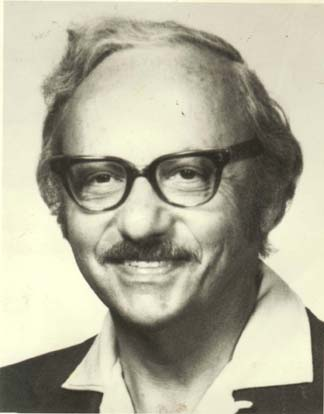
\includegraphics[scale=0.5]{figuren/lp/dantzig.jpg} 
     \caption{George B. Dantzig (1914--2005)}
    \label{fig:dantzig}
\end{figure}
In een interview uit 1986 vertelde Dantzig hoe hij zijn licentiaatsdiploma
in de wiskunde haalde zonder een thesis te schrijven. Blijkbaar
kwam hij eens te laat tijdens een les binnen. Op het bord stonden
twee problemen. Dantzig loste ze op en gaf ze een paar dagen later
af aan zijn professor. Hij verontschuldigde zich dat het zolang
geduurd had, maar deze huiswerkvragen vond hij toch iets moeilijker
dan gewoonlijk. Een paar weken later kreeg Dantzig zijn professor
op bezoek, die net zijn (correcte) oplossingen had bekeken. De
vragen aan het bord waren echter helemaal niet bedoeld als huiswerk,
maar het waren twee bekende onopgeloste problemen uit de statistiek!
De professor stelde ten slotte voor om deze twee antwoorden als
thesis te laten dienen.

Wat is nu juist een probleem uit de lineaire programmering? Een
poging tot \emph{definitie} is:

\begin{quote}
    Een lineair programmeringsprobleem bestaat erin een lineaire
doelfunctie van twee (of meer) onbekenden maximaal of minimaal
te maken. Deze onbekenden zijn onderworpen aan beperkingen die
(meestal)
de vorm aannemen van een stelsel lineaire ongelijkheden. Bijna
altijd eisen we dat onbekenden niet negatief mogen zijn.
\end{quote}

Volgend schema kan dienst doen als leidraad bij het oplossen
van oefeningen:

\begin{enumerate}
    \item  Vertaal het probleem naar wiskunde.
    \begin{itemize}
        \item  Maak indien mogelijk een overzicht van alle gegevens (bvb.\ in tabelvorm).

        \item  Bepaal wat de onbekende grootheden zijn. Geef ze
een naam.

        \item  Schrijf de beperkingen als lineaire ongelijkheden.

        \item  Zoek de doelfunctie (die minimaal of maximaal moet gemaakt
worden).
    \end{itemize}

    \item  Teken de \emph{geldige oplossingenverzameling}.
    \begin{itemize}
        \item  Schrijf de ongelijkheden in de standaardvorm (is
niet altijd nodig).

        \item  Teken de rechte die met elke ongelijkheid overeenkomt.

        \item  Bepaal het juiste halfvlak.
    \end{itemize}

    \item  Teken \'{e}\'{e}n van de \emph{doelfuncties} (geef een waarde
    aan $W$
of \emph{K}). Verschuif deze rechte evenwijdig tot ze net de geldige
oplossingenverzameling gaat verlaten. Bepaal  de co\"{o}rdinaten van het \emph{hoekpunt}.

    \item  Geef een \emph{volledig antwoord} op de vraag.
\end{enumerate}


%
%
%\newpage
%\section{De hoekpuntmethode}
%De methode die in beide voorbeelden hierboven werd gebruikt,
%is in essentie puur grafisch. In beide gevallen vonden we door
%de doelfunctie (isokosten- of isowinstrechte) te verschuiven,
%het optimale punt dat toch nog net tot de verzameling van alle
%geldige oplossingen behoorde.
%
%Het is niet toevallig dat die optimale oplossing telkens een
%\emph{hoekpunt} was van de verzameling geldige oplossingen. De `hoekpunt'-methode
%maakt hier dankbaar gebruik van. Ze steunt op volgende stelling
%(die we zonder bewijs geven).
%
%
%\subsection{Fundamentele stelling van de lineaire programmering}
%Als de geldige oplossingenverzameling begrensd is (een veelhoek,
%zoals in het maximalisatie-vraagstuk uit paragraaf~\ref{sec.maxprob}), dan heeft de doelfunctie zowel een maximum als
%een minimum. Beiden worden bereikt in \'{e}\'{e}n van de hoekpunten
%van de geldige oplossingenverzameling.
%
%Als deze verzameling niet begrensd is (zoals in het
%minimalisatievoorbeeld uit paragraaf~\ref{sec.minprob}),
%bestaat de mogelijkheid dat de doelfunctie geen minimum of geen
%maximum bereikt. Maar \emph{als} er wel een minimum of maximum bestaat,
%zal het met zekerheid voorkomen in een hoekpunt!
%
%
%
%\subsection{Voorbeeld 1 met de hoekpuntmethode}
%We hernemen in figuur~\ref{fig:hoekpuntmethode} even de
%tekening van de geldige oplossingenverzameling.
%\begin{figure}[htbp]
%    \centering
%\begin{tikzpicture}[scale=0.5]
%\draw[->] (-1,0) -- (17,0) node[right] {$x$};
%\draw[->] (0,-1) -- (0,17) node[above] {$y$};
%\foreach \x in {2,4,...,16}
%	\draw[shift={(\x,0)}] (0pt,2pt) -- (0pt,-2pt) node[below] {\footnotesize $\x$};
%\foreach \y in {2,4,...,16}
%	\draw[shift={(0,\y)},color=black] (2pt,0pt) -- (-2pt,0pt) node[left] {\footnotesize $\y$};
%\node [below left] at (0,0) {\footnotesize 0};	
%%	\fill[pattern=north east lines, pattern color=gray]  (-1,12.2) -- (5,11)-- (10,6) -- (10,-1) -- (18,-1) -- (18,17) -- (-1,17) -- cycle;
%\draw[dotted](-1,12.2) -- (14,9.2);
%\draw[dotted](10,-1) -- (10,12);
%\draw[dotted](-1,17) -- (17,-1);
%\draw[very thick, red] (0,0) -- (10,0) -- (10,6) -- (5,11) -- (0,12) -- cycle;
%\node (A) [above right, donkergroen] at (0,0) {A(0,0) $\Rightarrow W=0$};
%\filldraw [donkergroen] (0,0) circle (4pt);
%\node (B) [above right, donkergroen] at (10,0) {B(10,0) $\Rightarrow W=250$};
%\filldraw [donkergroen] (10,0) circle (4pt);
%\node (C) [above right, donkergroen] at (10,6) {C(10,6) $\Rightarrow W=700$};
%\filldraw [donkergroen] (10,6) circle (4pt);
%\node (D) [above right, donkergroen,draw,rounded corners,thick] at (5,11) {D(5,11) $\Rightarrow W=950$};
%\filldraw [donkergroen] (5,11) circle (4pt);
%\node (E) [above right, donkergroen] at (0,12) {E(0,12) $\Rightarrow W=900$};
%\filldraw [donkergroen] (0,12) circle (4pt);
%\end{tikzpicture}
%    \caption{Hoekpuntmethode}
%    \label{fig:hoekpuntmethode}
%\end{figure}
%
%Deze gesloten veelhoek heeft vijf hoekpunten. Het enige wat we nu
%moeten doen is elk hoekpunt invullen in de doelfunctie.
%Vermits de geldige oplossingenverzameling begrensd is, ben je
%zeker dat \'{e}\'{e}n van de hoekpunten de maximale, en \'{e}\'{e}n de
%minimale waarde van de doelfunctie zal opleveren.
%
%\begin{table}[hbp]
%    \centering
%    \caption{Winst in elk hoekpunt}
%    \begin{tabular}{cr}
%        \toprule
%        Hoekpunt & Winst  \\
%        \midrule
%        A(0,0) & 0  \\
%        B(0,12) & 900  \\
%        C(5,11) &   950\\
%        D(10,6) &700 \\
%        E(10,0) & 250  \\
%        \bottomrule
%    \end{tabular}
%    \label{tbl:hoeken}
%\end{table}
%
%Antwoord: De \emph{minimale} winst bereikt de boer als hij geen dieren
%houdt (\euros 0). De \emph{maximale} opbrengst krijgt hij
%door vijf kippen en elf schapen te houden (\euros 950).


\newpage
\section{Uitzonderlijke situaties}
Volgende puntjes komen bij echte praktische vraagstukken zelden
voor. Als ze dan toch de kop opsteken, wijst dit dikwijls op \emph{een
foutieve formulering van het lineair programmeringsprobleem}.
Voor een computerprogramma moeten deze uitzonderlijke situaties
toch bekeken worden.



\subsection{G\'{e}\'{e}n punten in de geldige oplossingenverzameling}
Bekijk volgend lineair programmeringsvraagstuk: maximaliseer
\begin{displaymath}
    P=x+2y
\end{displaymath}
Met als beperkingen
\begin{eqnarray*}
    x+y & \geqslant & 3  \\
    x+2y & \leqslant & 2  \\
    2x+y & \leqslant & 2  \\
    x \mbox{ en } y & \geqslant & 0
\end{eqnarray*}
Maak zelf een tekening voor deze opgave. Als we dit systeem van vijf ongelijkheden proberen op te lossen,
moeten we alle punten zoeken die niet in gearceerd gebied liggen. Je
merkt op de tekening dat er geen enkel dergelijk punt bestaat.



\subsection{Meer dan \'{e}\'{e}n optimaal punt}
Als de doelfunctie evenwijdig loopt met \'{e}\'{e}n van de grenslijnen
van de geldige oplossingenverzameling, is elk punt op deze grenslijn
een optimaal punt. Bekijk even volgende opgave:
Maximaliseer
\begin{displaymath}
    P=2x+y
\end{displaymath}
Met als beperkingen
\begin{eqnarray*}
    2x+y & \leqslant & 2  \\
    x+2y & \leqslant & 2  \\
    x \mbox{ en }y & \geqslant & 0
\end{eqnarray*}
Maak opnieuw zelf de tekening.



\subsection{Onbegrensde oplossingenverzameling bij maximalisatie}
Maximaliseer:
\begin{displaymath}
    P=x+y
\end{displaymath}
Met als beperkingen
\begin{eqnarray*}
    -x+y & \leqslant & 1  \\
    y & \leqslant & 2  \\
    x \mbox{ en } y & \geqslant & 0
\end{eqnarray*}
Maak de figuur en laat zien dat je $P$ zo groot kan maken als je maar wil.


% \newpage
\section{Meerdere onbekenden}
In dit hoofdstukje beperkten we ons tot problemen met twee onbekenden
(bvb.\ het aantal kippen en het aantal schapen).

Er bestaan echter ook methodes om lineaire programmeringsvraagstukken
met meerdere onbekenden op te lossen (bvb.\ de simplexmethode).
Dit komt in het tweede semester aan bod in het OPO Toegepaste Wiskunde 2.

%%%%%%%%%%%%%%%%%%%%%%%%%%%%%%%%%
% Laatste aanpassing: 
% 5/1/14 [Jan]: oplossing oefening loften aangepast (suggestie Inge)
%
% 26/06/13 [Greetje]: Oefeningen van Leentje toegevoegd
% 18/2/12 [Jan]: Oef 7 aangepast
%
% 2/2/11 [Greetje]: nieuwe oefeningen toegevoegd. Formulering van sommige oefeningen aangepast.
%
% 14/09/10 [Greetje]: opgaven in 3 veranderlijken verwijderd. Herhalingsvragen weggelaten.
%
% 11/9/07 [Jan]: enkele fouten verbeterd
%          
% 14/9/05 [Jan]: vraag is 10 stoelen (i.p.v. 30)
%
% 8/09/01 door Greetje
%   correcties van Roos en Roby
%
% nieuwe aanpassing: 8/06/02 door Roos  %
%  nieuwe opgaven en volgorde veranderd       %
%%%%%%%%%%%%%%%%%%%%%%%%%%%%%%%%%

%\chapter{Oefeningen op lineaire programmering}
\section{Oefeningen}
\begin{oef}
De Indische regering kondigt een ambitieus plan aan om in
     ieders voedselbehoefte te kunnen voorzien op basis van rijst en
     sojascheuten. E\'{e}n kopje ongekookte rijst kost \euros{0,20} en bevat
     15 gr eiwitten, 810 calorie\"{e}n en $\frac{1}{9}$ mg vitaminen
     B2. E\'{e}n kopje sojascheuten kost \euros{0,40} en
     levert 22,5 gr eiwitten, 270 calorie\"{e}n en $\frac{1}{3}$ mg
     B2. Veronderstel dat de minimale dagelijkse
     behoeften er als volgt uitzien: 90 gr eiwitten, 1620 calorie\"{e}n
     en 1 mg vitamine B2.
 Hoe ziet het goedkoopste
     dieet dat voldoet aan de minimale behoeften eruit?
     \begin{opl}
     De goedkoopste oplossing (figuur~\ref{fig:oplrijstsoja}) die aan alle beperkingen voldoet is drie kopjes rijst en twee kopjes sojascheuten, met een kostprijs van \euros{1,40}. 
     \begin{figure}[hbtp]
\centering
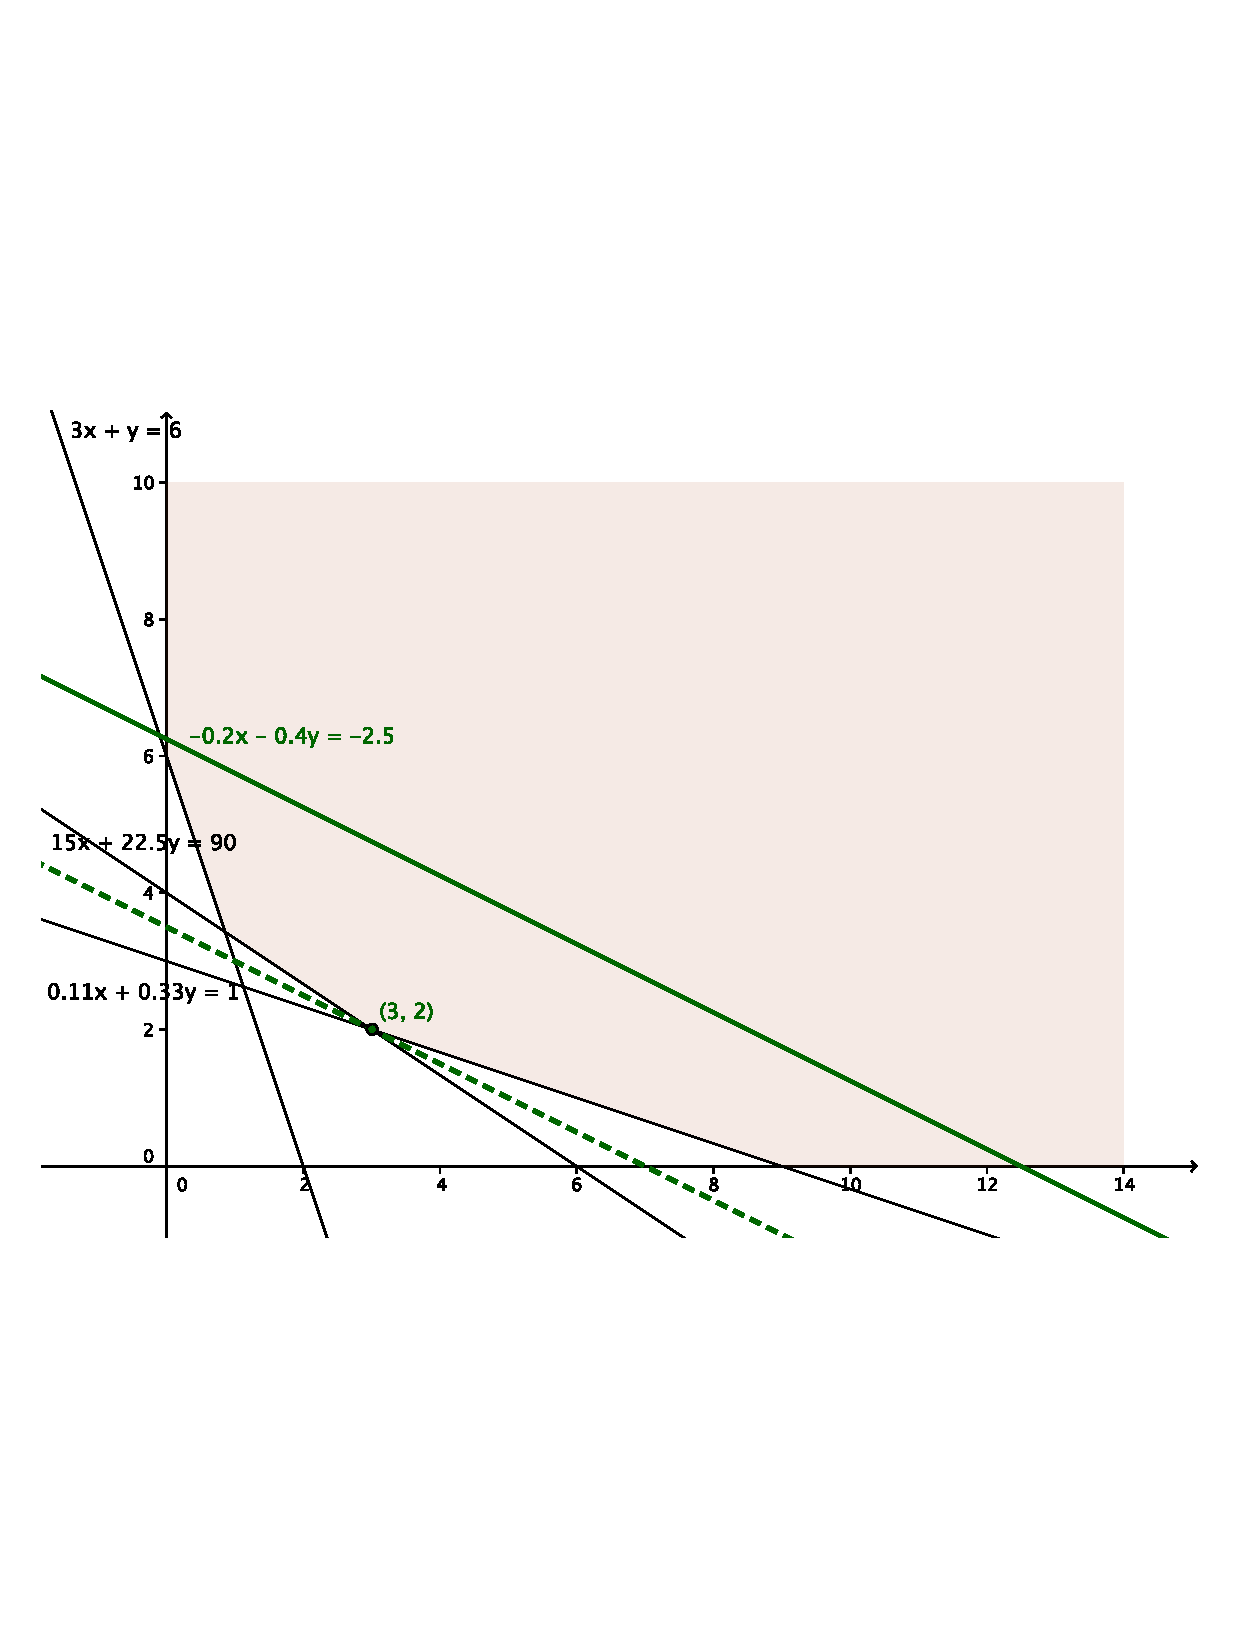
\includegraphics[width=0.8\textwidth]{oefeningen/FigurenLP/OefRijstSoja.pdf}
\caption{Optimaal punt is drie kopjes rijst en twee kopjes soja}
\label{fig:oplrijstsoja}
\end{figure}

     \end{opl}
\end{oef}
 
\begin{oef}
In een bedrijf worden nieuwe archiefkasten aangekocht. Er
     is keuze tussen 2 types met verschillende afmetingen en
     functies. Type A kost \euros{150} en is \SI{60}{\cm} diep, \SI{40}{\cm} breed en
     \SI{1}{\m} hoog. Type B kast kost het dubbele van A maar is \SI{45}{\cm}
     diep, \SI{80}{\centi\meter} breed en \SI{1,5}{\meter} hoog. Voor elke type A kast moeten
     minstens 2 kasten van type B geplaatst worden. De totale
     grondoppervlakte die in het bedrijf moet ingenomen worden door
     archiefkasten is minstens \SI{3,84}{\square\meter}. Er is in totaal \euros{7500}
     voorzien voor de aankoop. Hoeveel kasten van elk type moeten
     er aangekocht worden om de kostprijs zo laag mogelijk te houden? 
     \begin{opl}
     Vier kasten van type A en acht kasten van type  B leveren de goedkoopste prijs van \euros{3000} en voldoen aan alle voorwaarden (figuur~\ref{fig:kastenAB}).
          \begin{figure}[hbtp]
\centering
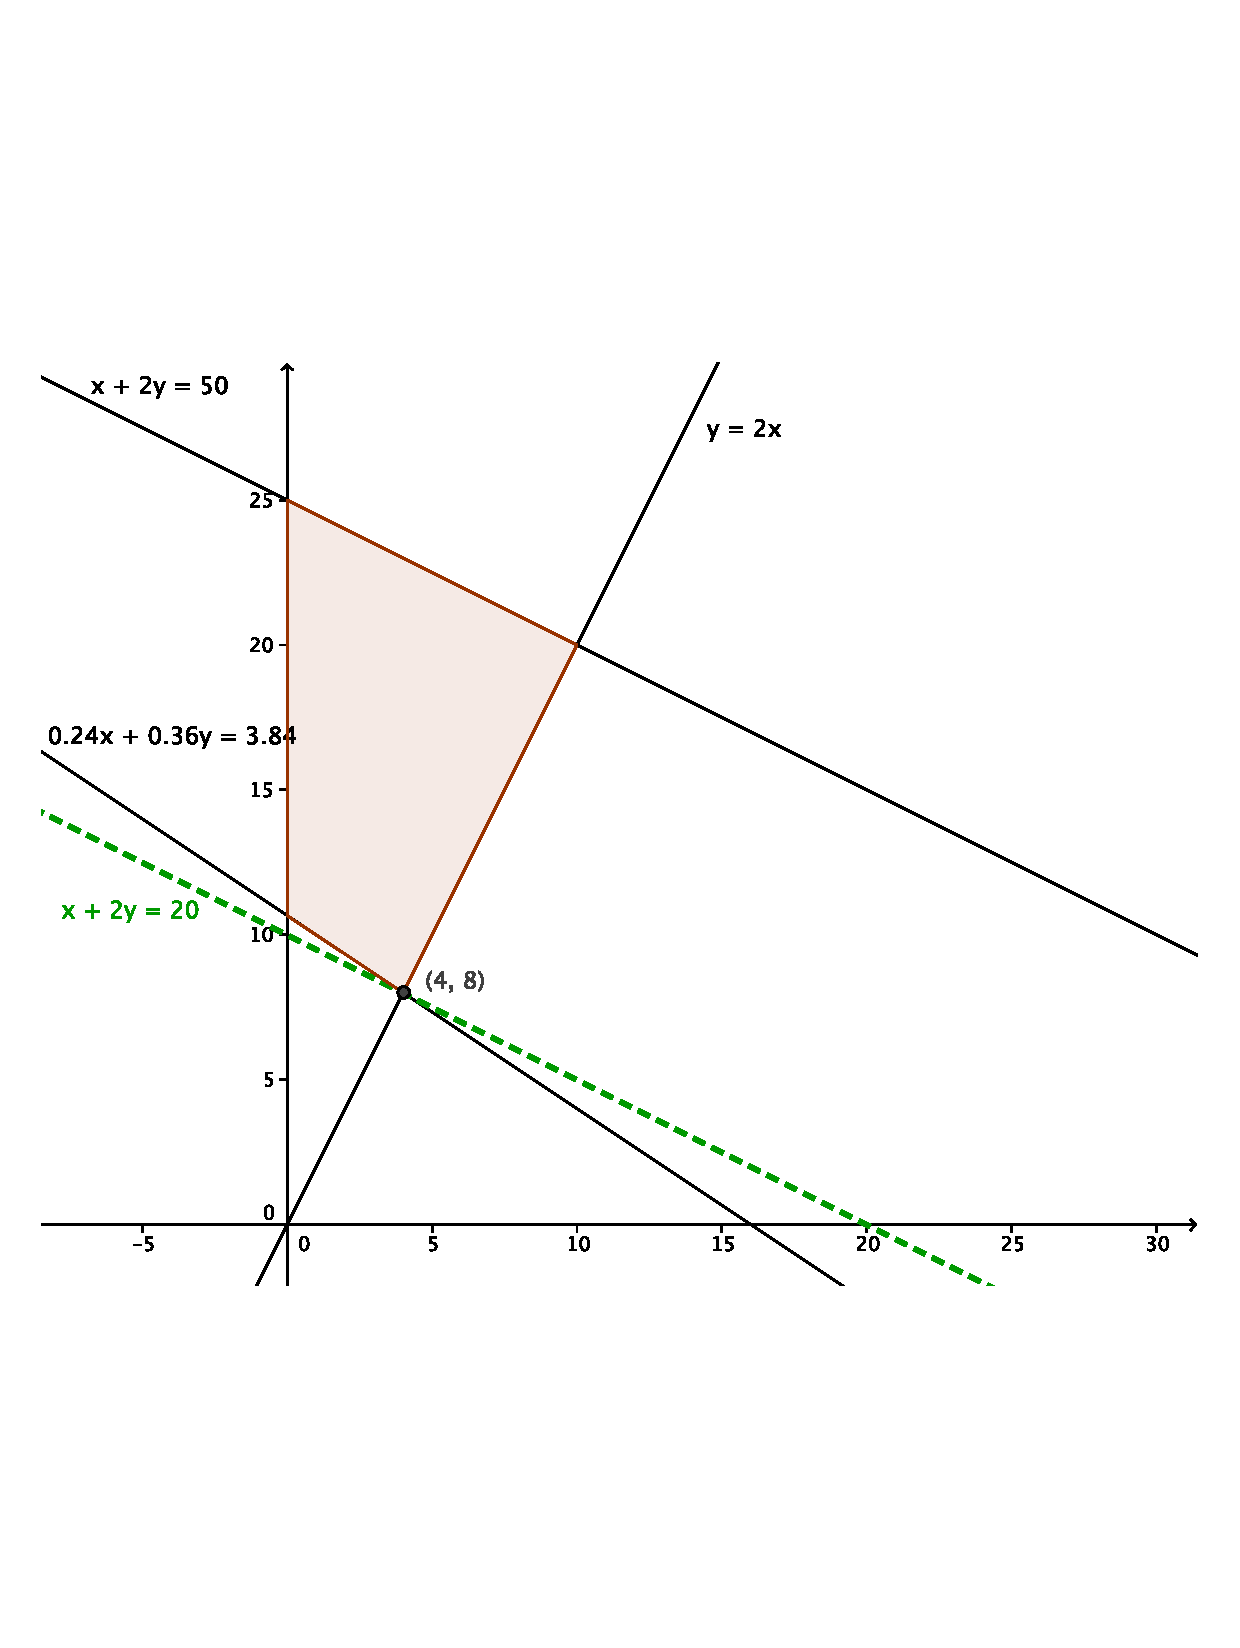
\includegraphics[width=0.8\textwidth]{oefeningen/FigurenLP/OefkastenAB.pdf}
\caption{Optimaal punt is vier kasten A en acht kasten B}
\label{fig:kastenAB}
\end{figure}
     \end{opl}
\end{oef}
     
     
   
\begin{oef}
Het departement G\&T wordt verkozen tot `Departement van het
    jaar'. Als beloning mogen alle personeelsleden en studenten -- in
    totaal 2000 mensen -- gratis voor  \'{e}\'{e}n week op reis naar
    Kreta. `Cobol Airlines' zorgt voor het transport. 
\begin{figure}[h]
\centering
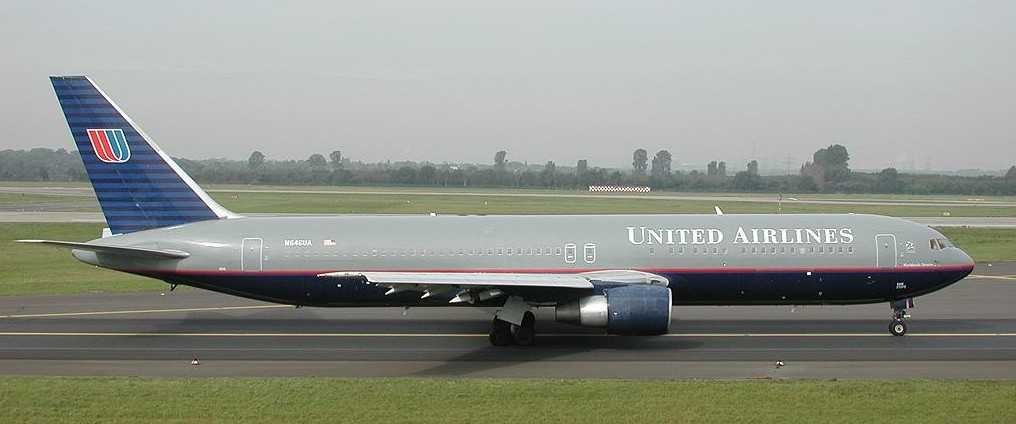
\includegraphics[width=0.8\textwidth]{oefeningen/FigurenLP/Boeing-767.jpg}
\caption{Boeing 767-300}
\end{figure}
    Deze
    luchtvaartmaatschappij beschikt over een vloot van Fokkers en
    Boeings 767. De Fokker heeft een capaciteit van 80 passagiers,
    heeft 3 stewards aan boord en kost per vlucht \euros{20\,000}. De
    Boeing 767 kan 240 personen meenemen, vraagt 4 Stewards en kost
    \euros{100\,000} per vlucht.`Cobol Airlines' beschikt over 50
    stewards. Er moeten minstens evenveel Fokkers als Boeings
    ingezet worden voor het vervoer van deze 2000 mensen.
Wat is de samenstelling van toestellen zodat 
	de reis zo goedkoop mogelijk
    wordt? Hoeveel kost de reis?   
    \begin{opl}
    Tien Fokkers en vijf Boeings leveren de goedkoopste transportoplossing (figuur~\ref{fig:deptjaar}) met een kostprijs van \euros{700\,000}.
              \begin{figure}[hbtp]
\centering
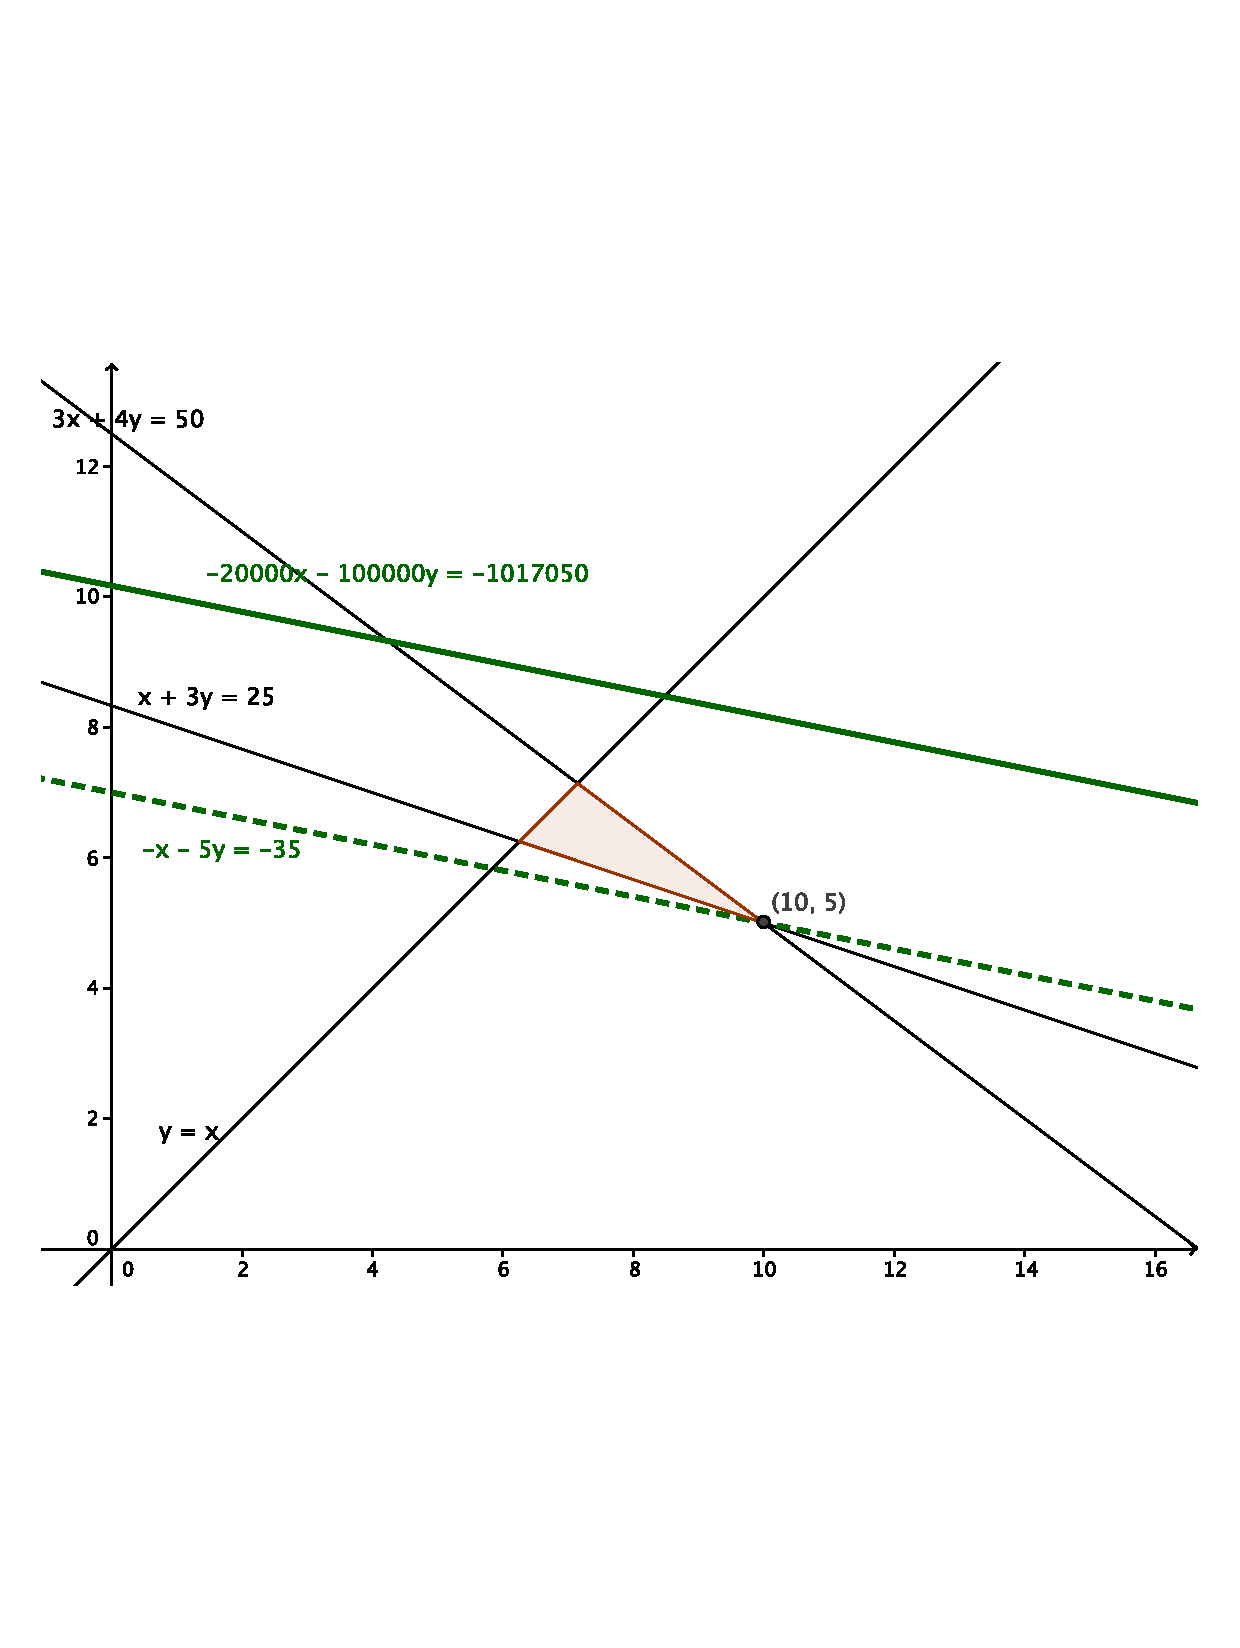
\includegraphics[width=0.8\textwidth]{oefeningen/FigurenLP/OefDepvhjaar.pdf}
\caption{Optimaal punt is 10 Fokkers en 5 Boeings}
\label{fig:deptjaar}
\end{figure}
    \clearpage
    \end{opl}
\end{oef}      

\begin{oef}
Artsen zonder Grenzen plannen een konvooi om de
     noodlijdende bevolking van een vluchtelingenkamp in Afghanistan te 
     bevoorraden met tenten en dekens, zodat de mensen de winter kunnen 
     doorkomen. Per tent worden minstens drie dekens geleverd. Het totale laadvermogen van alle voertuigen samen is 
     10 ton. Een tent weegt 2 kg en een deken 1 kg. Er zijn slechts 8000 dekens beschikbaar. Met een tent kan men 
     5 vluchtelingen helpen, met een deken slechts \'{e}\'{e}n 
     vluchteling. Hoeveel tenten en dekens moet men leveren om zoveel 
     mogelijk mensen te helpen? 
     \begin{opl}
     Met 2000 tenten en 6000 dekens kunnen in totaal 16\,000 mensen geholpen worden (figuur~\ref{fig:AZG}).
                   \begin{figure}[hbtp]
\centering
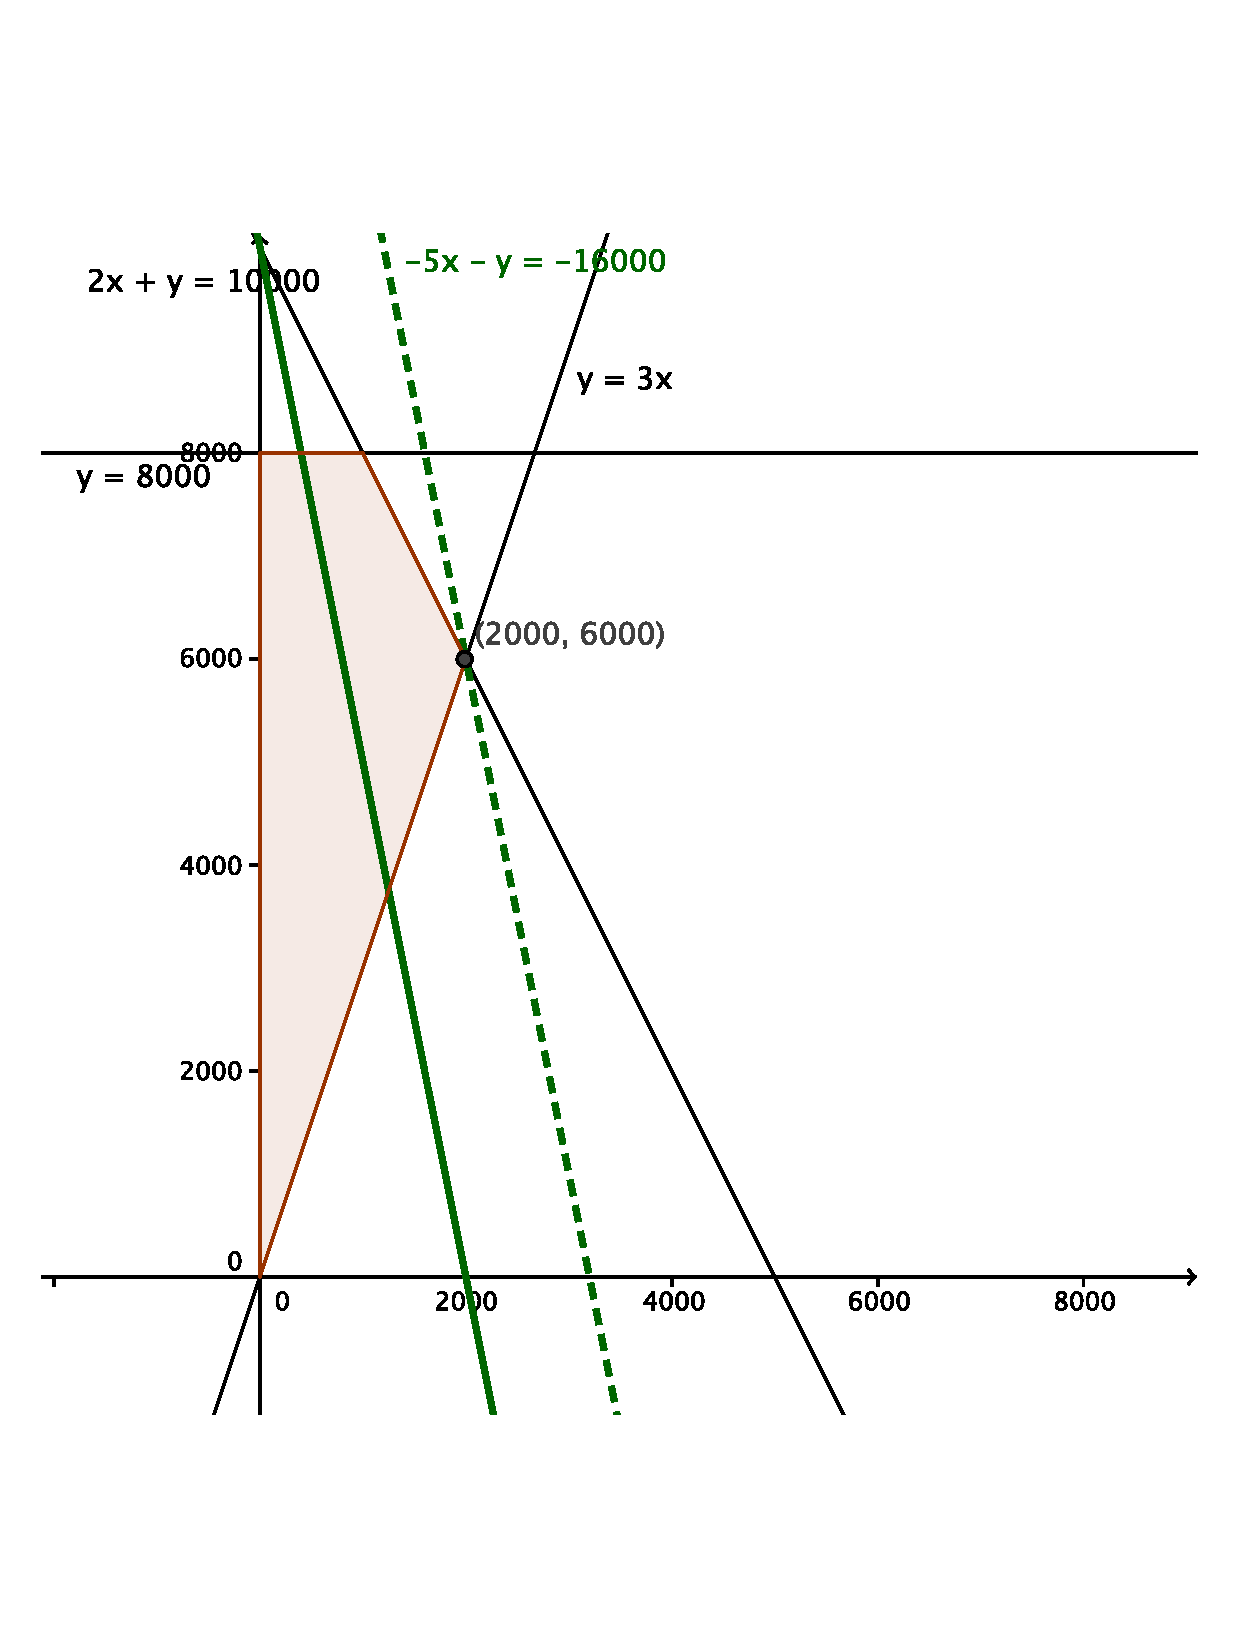
\includegraphics[width=0.7\textwidth]{oefeningen/FigurenLP/OefAZG.pdf}
\caption{Optimaal punt is 2000 tenten en 6000 dekens}
\label{fig:AZG}
\end{figure}
     \end{opl}
\end{oef}
     
\begin{oef}
In een speelgoedfabriek worden Woody
en Buzz Lightyear poppen gemaakt. 
\begin{figure}[ht]
  \centering
    
\includegraphics[scale=0.5]{oefeningen/FigurenLP/Buzz-Woody.jpg}
\end{figure}
Omwille van beperkingen van machines
kunnen er dagelijks in totaal maximaal 100 poppen gemaakt worden. De
directie van de fabriek heeft besloten om minstens 10 Buzz Lightyear
poppen en hoogstens 80 Woody poppen te maken per dag. 
De milieubijdrage
voor een Buzz Lightyear pop is 2 euro terwijl die maar de helft
bedraagt voor een Woody pop. De directie wil dagelijks niet meer dan 130
euro voorzien als milieubijdrage. Wegens de grotere populariteit van
Woody, worden er minstens evenveel Woody poppen gemaakt als Buzz
Lightyear poppen. Het bedrijf maakt een winst van 20 euro per Woody pop
en 10 euro per Buzz Lightyear pop. \begin{enumerate}
	\item Bepaal de optimale dagelijkse productie van Woody en Buzz
Lightyear poppen zodat het bedrijf een maximale winst heeft.
(\textit{Je mag hierbij van uitgaan dat alle geproduceerde poppen ook
effectief zullen worden verkocht en dus winst opleveren.}) Vermeld
duidelijk en gedetailleerd welke stappen je hebt gevolgd om tot je
oplossing te komen.
	\item  Bereken de bijhorende maximale winst.
\end{enumerate}
\end{oef}
  
\begin{oef}
Een boer wil hoogstens 40 ha van zijn land bebouwen met
     ma\"{i}s en aardappelen. Uit ervaring weet hij dat per ha ma\"{i}s
     $3$ dagen
     (hand)werk mag gerekend worden en per ha aardappelen 10 dagen.
     Volgens zijn werkschema kan hij hoogstens 240 werkdagen besteden
     aan het met de hand bewerken van ma\"{i}s en aardappelen. De machines
     bezit hij samen met andere boeren zodat hij slechts gedurende 47
     extra dagen over de nodige machines kan beschikken. Voor de 
     ma\"{i}s kan men per dag  \'{e}\'{e}n ha bewerken met 
     machines en voor 
     de aardappelen bewerkt men per dag $\frac{2}{3}$ van een ha. 
     Uiteindelijk  moet het aandeel van de ma\"{i}s minstens  \'{e}\'{e}n
     derde van de totale bewerkte oppervlakte zijn. De opbrengst
     per ha
     voor ma\"{i}s \euros{1000} is en die van aardappelen \euros{3000}.
Bepaal de verdeling van bewerkte oppervlakte ma\"{i}s en
     aardappelen die een maximale opbrengst levert. Bereken ook die
     opbrengst. 
     \begin{opl}
     20 ha ma\"is, 18 ha aardappelen
     \end{opl}
\end{oef}
     
     
     
     
\begin{oef}
In een bedrijf produceert men tafels en stoelen. Voor de
     productie van \'{e}\'{e}n tafel is 3 maal zoveel hout nodig als
     voor de productie van \'e\'en stoel. Er is in het bedrijf voldoende
     hout aanwezig om per week 45 stoelen te maken. Een stoel vraagt echter
     heel wat afwerking, zodat er voor het maken van \'{e}\'{e}n
     stoel 2 maal zoveel personeel nodig is als voor een tafel. Het
     bedrijf beschikt over net voldoende personeel om 20 stoelen af te
     werken per week. De vraag naar tafels en stoelen samen, per week,
     is 10 stuks, zodat het bedrijf per week minstens 10 meubelstukken zal produceren. De winst per tafel is \euros{125} en die per stoel is
     \euros{75}. Hoeveel tafels en stoelen moet men produceren om de
        winst zo groot mogelijk te maken? Hoeveel bedraagt de winst?
        \begin{opl}
        10 tafels en 15 stoelen (figuur~\ref{fig:tafelstoelen}) leveren de grootste winst, nl \euros{2375}.
        \begin{figure}[hbtp]
\centering
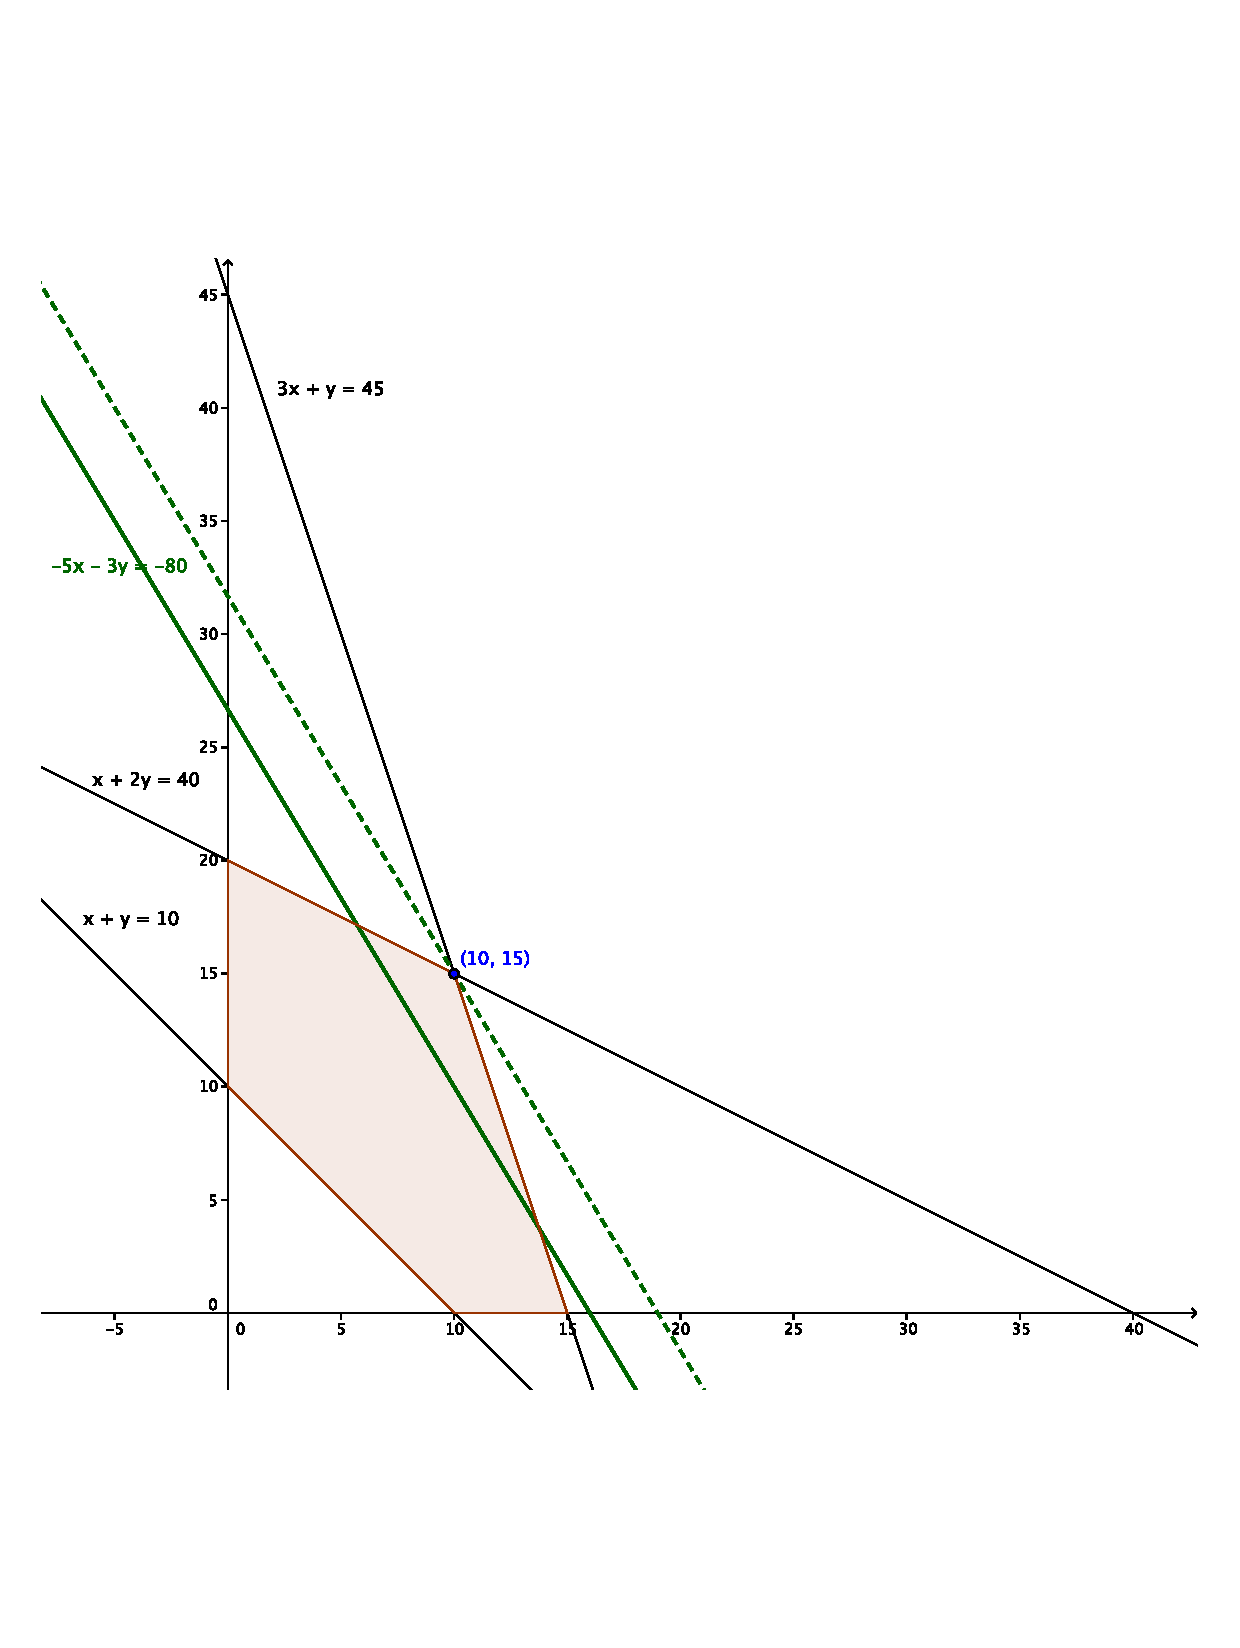
\includegraphics[width=0.8\textwidth]{oefeningen/FigurenLP/Oef7.pdf}
\caption{10 tafels en 15 stoelen leveren de grootste winst}
\label{fig:tafelstoelen}
\end{figure}
\clearpage
        \end{opl}
\end{oef}

     
\begin{oef}
Een bedrijf produceert 2 types containers.
     Voor de productie van 
    \'{e}\'{e}n container van type A is driemaal zoveel personeel 
    nodig als voor \'{e}\'{e}n container van type B. Het bedrijf 
    beschikt over voldoende personeel om 120 containers van type B te 
    maken per dag. Voorts vereist \'{e}\'{e}n container van type B 
    tweemaal zoveel staal als \'{e}\'{e}n container van type A. Er is 
    in het bedrijf voldoende staal aanwezig om per dag 60 containers 
    van type A te maken. De winst per container van type A is \euros {2500} 
    en die per container van type B is \euros{1000}. Er is elke dag 
    vraag naar \emph{minstens} 15 containers van beide types samen. Het 
    aandeel van containers van type A is minstens \'{e}\'{e}n  vierde 
    van de dagelijkse productie van beide types containers \emph{samen}. 
    \emph{Hoeveel} containers van type A en hoeveel van type B moet 
    het bedrijf produceren om de winst zo groot mogelijk te maken?
    \begin{opl}
    De maximale winst (\euros{102\,000}) wordt bereikt bij de productie van 36 containers van type A en 12 containers van type B (figuur~\ref{fig:containersAB}).
            \begin{figure}[hbtp]
\centering
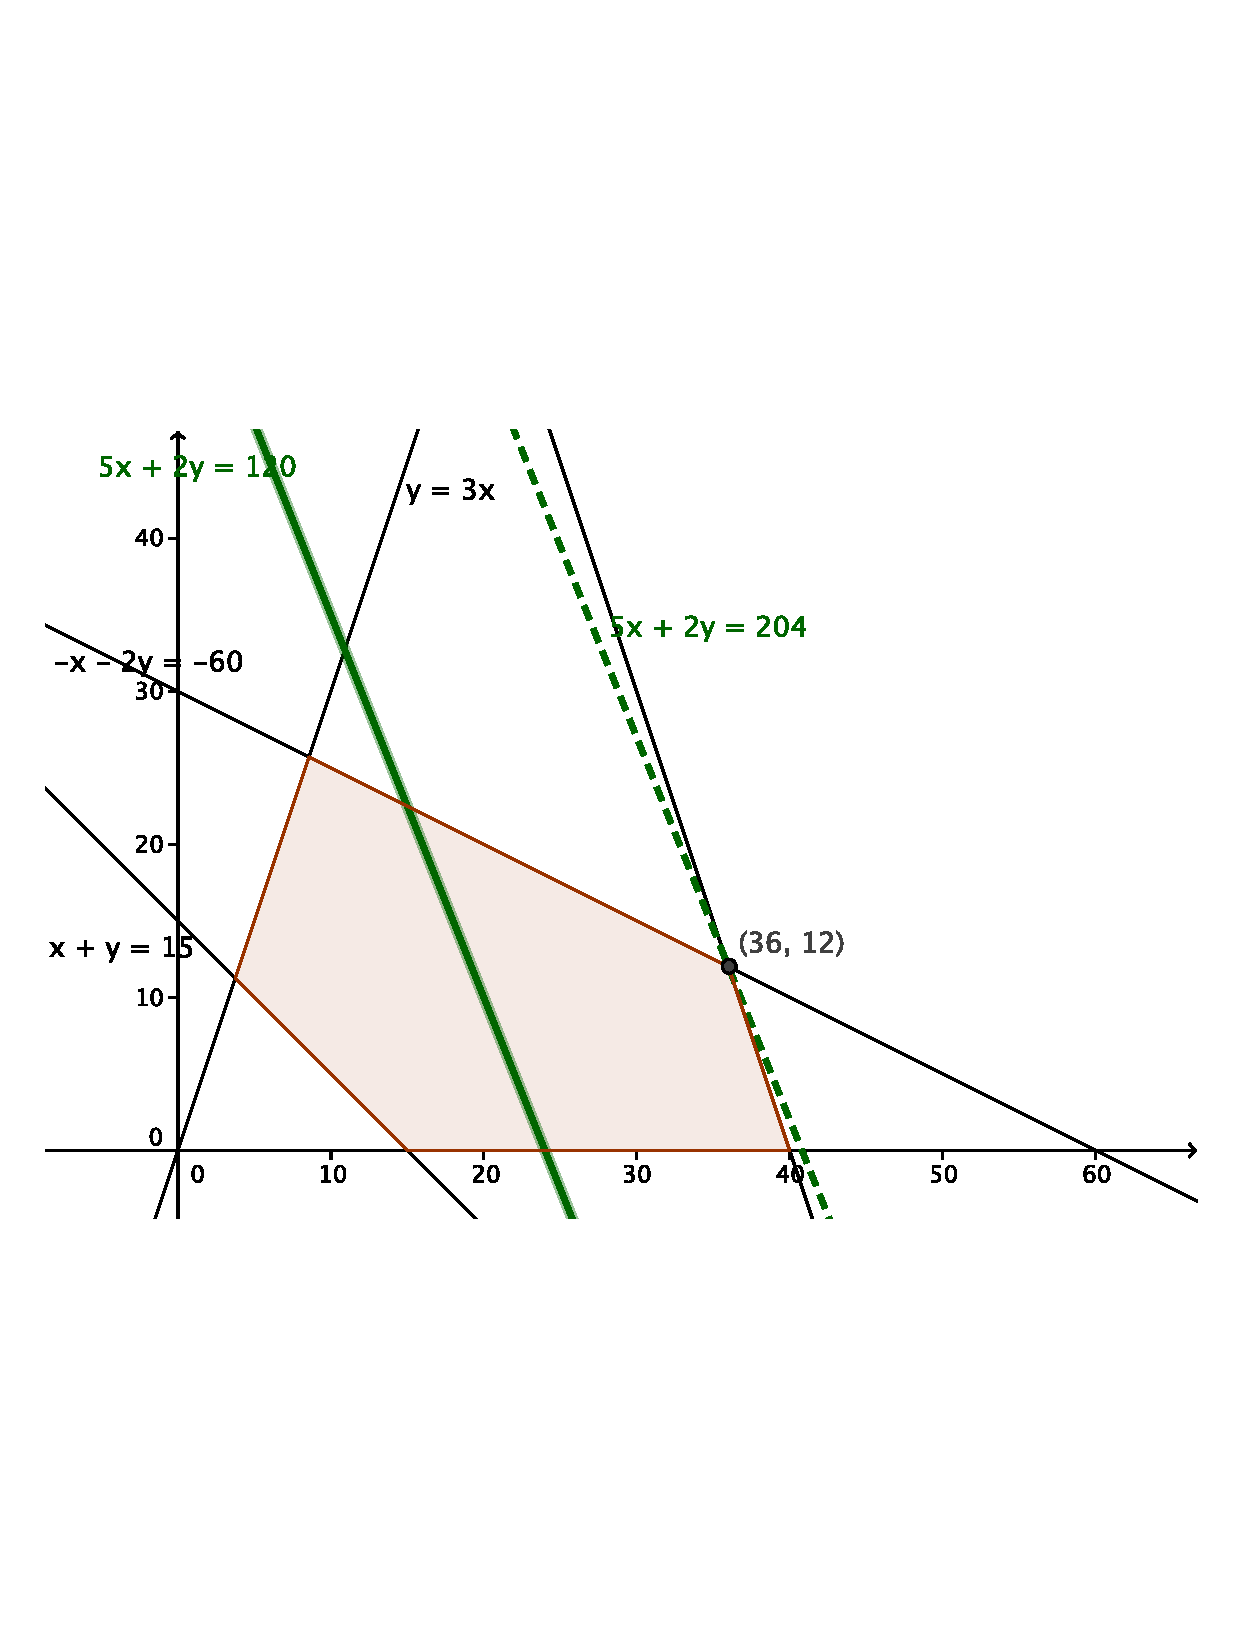
\includegraphics[width=0.8\textwidth]{oefeningen/FigurenLP/OefcontainersAB.pdf}
\caption{De grootste winst is bij 36 containers A en 12 containers B}
\label{fig:containersAB}
\end{figure}
    \end{opl}
\end{oef}

\begin{oef}
Een fabriek produceert metalen platen en buizen.
     Het aantal machines voor deze productie laat toe om maximaal 35
     ton platen \emph{of} 70 ton buizen per maand te maken. Hiervoor zijn 80
     arbeiders beschikaar. E\'en man kan per maand 1 ton platen \emph{of} 500
     kg buizen verwerken. De buizen vereisen een nabehandeling in een
     andere afdeling waar slechts 35 ton per maand kan afgewerkt
     worden.   De opbrengst voor de fabriek op \'e\'en ton platen en
     \'e\'en ton buizen is respectievelijk \euros{2500} en
     \euros{2000}. Bepaal  de optimale
     productie waardoor de fabriek een maximale opbrengst bekomt. 
     \begin{opl}
     Een maandproductie van 20 ton platen en 30 ton buizen (figuur~\ref{fig:platenbuizen}) levert de maximale winst van \euros{110\,000}.
                 \begin{figure}[hbtp]
\centering
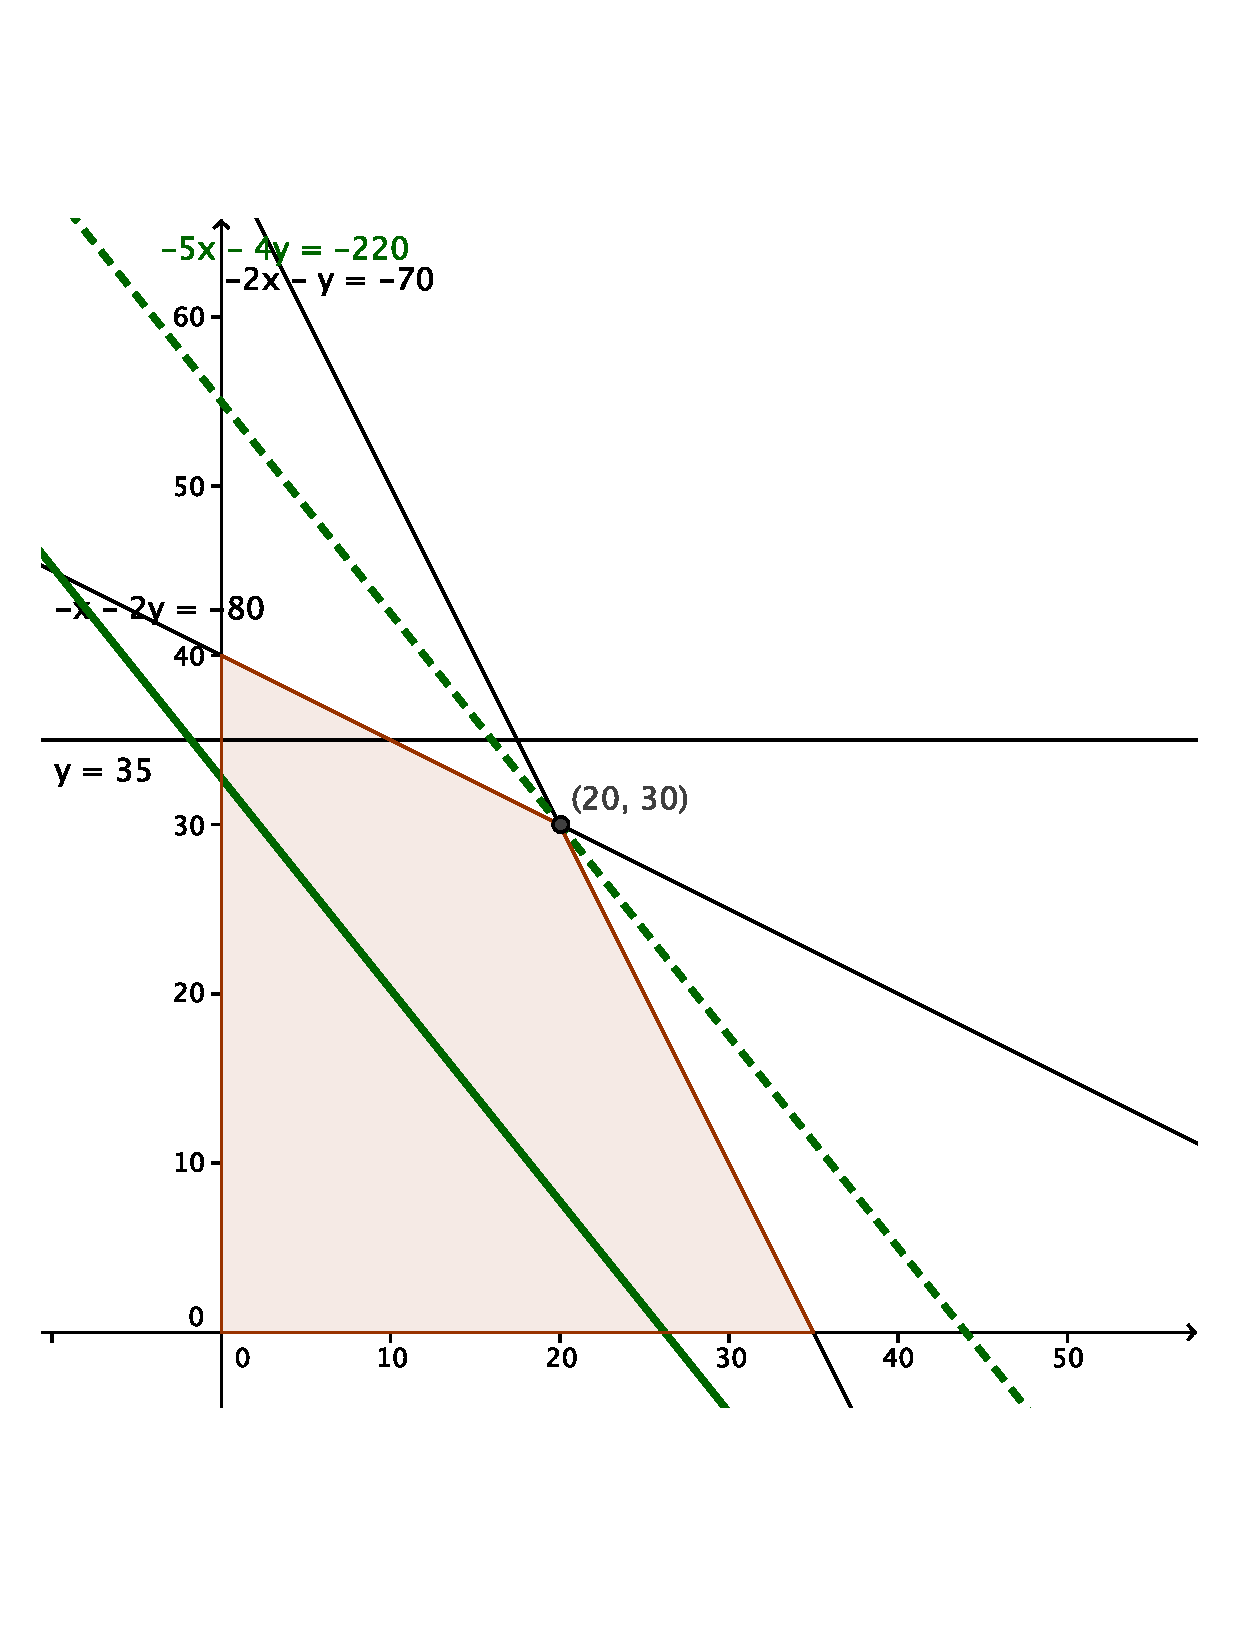
\includegraphics[width=0.8\textwidth]{oefeningen/FigurenLP/OefPlatenBuizen.pdf}
\caption{Maximale winst bij 20 ton platen en 30 ton buizen}
\label{fig:platenbuizen}
\end{figure}
\clearpage
     \end{opl}
\end{oef}
     


\begin{oef}
Een bioscoopzaal draait voorlopig alleen 
    `The lord of de Rings (LR) en `Harry Potter en de steen der wijzen' (HP). Bij 
     voorstellingen van LR laat men maximaal 100 volwassenen en 50 
     kinderen toe (inkomprijs \euros{8} resp.\ \euros{6}). Bij HP is dat 
     40 volwassenen en 160 kinderen (inkomprijs \euros{7} resp.\ 
     \euros{4}).  De onkosten 
     (personeel, rechten, apparatuur\ldots) voor 
     een voorstelling van LR bedragen \euros{200} voor HP \euros{120}.  De 
     totale winst van alle voorstellingen samen moeten minstens 
     \euros{21600} bedragen. Het poetswerk na een vertoning van LR duurt 
     10 minuten en bij HP 20 minuten. Het poetspersoneel mag in totaal  
     maximum 7.5 uren werken. De filmdistributeur bepaalt dat het aantal 
     vertoningen van LR  maximum 30 bedraagt en minstens 
     evenveel als het aantal vertoningen van HP. We veronderstellen 
          dat alle vertoningen vol geboekt zijn.
     Hoeveel voorstellingen van elke film moet men geven opdat het aantal 
     kinderen dat naar de film kan zo groot mogelijk is? 
     \begin{opl}
     15 voorstellingen van elke film
     \end{opl}
\end{oef}
     

\begin{oef}
De directie van een pretpark buigt zich over de uitbreiding van het
parkeerterrein met een aanpalend stuk grond. Op de parking kunnen zowel auto's als autobussen parkeren. Voor de autobussen worden geen speciale plaatsen voorzien: zij nemen gewoon 3 autoparkeerplaatsen in.  Er is ruimte voor 75
personenauto's.  Er worden maximaal 10 bussen toegelaten op de parking. 
Per bus moeten minstens 3 auto's toegelaten worden en mogen er maximaal 8 auto's parkeren.  Per dag levert een auto \euros{4}
parkeergeld op, een autobus \euros{15}. Hoeveel auto's en bussen moeten er op de parking parkeren opdat de opbrengst per dag maximaal zou zijn? 
\begin{opl}
Als de parking dagelijks 45 auto's en 10 bussen ontvangt (figuur~\ref{fig:autobussen}), is de opbrengst maximaal (\euros{330}).
                 \begin{figure}[hbtp]
\centering
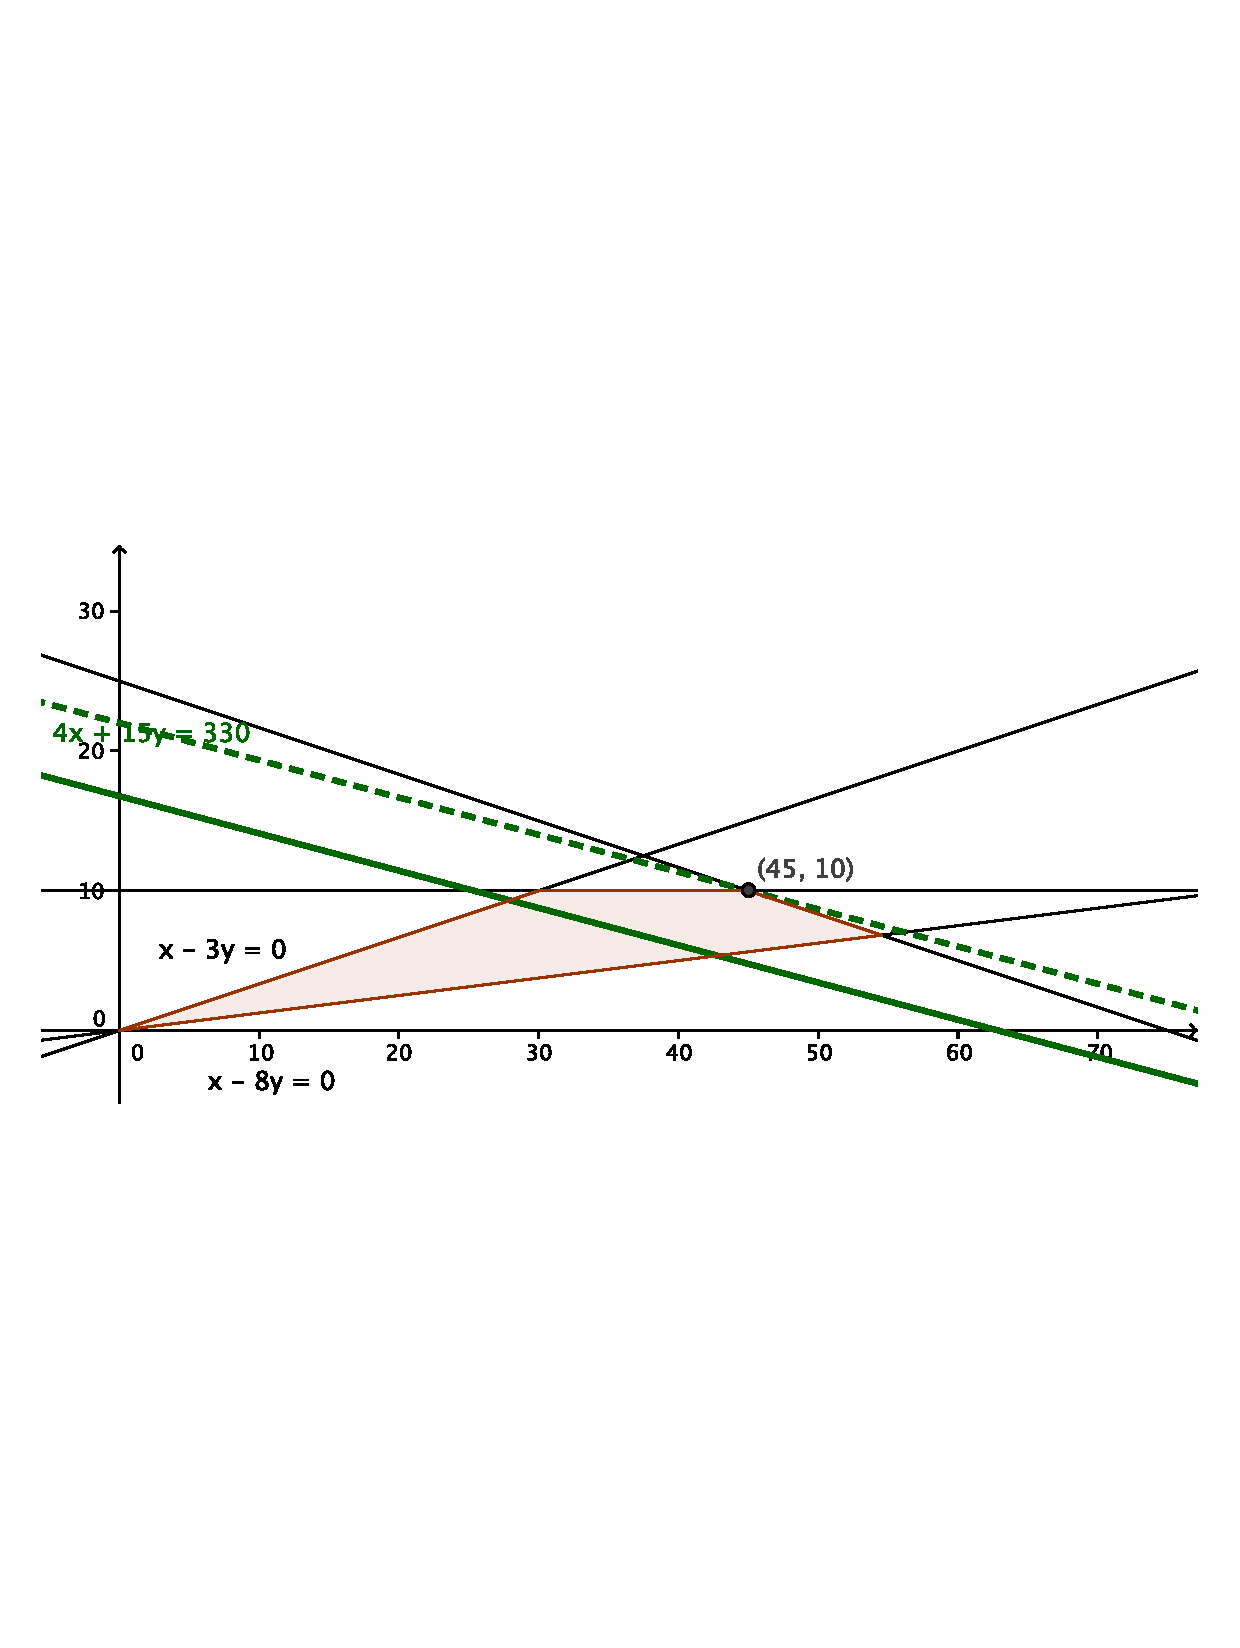
\includegraphics[width=0.8\textwidth]{oefeningen/FigurenLP/Oefautosbussen.pdf}
\caption{Maximale parkingopbrengst bij 45 auto's en 10 bussen}
\label{fig:autobussen}
\end{figure}
\end{opl}
\end{oef}

\begin{oef}
Voor een sponsoractie op school vult Anne potjes met vanille- en chocoladepudding. 
Haar moeder heeft 40 potjes die ze kan vullen 
(maar ze moeten niet allemaal gevuld worden).
Anne heeft de juf beloofd om minstens 25 potjes mee te brengen.
Ze denkt dat meer mensen vanillepudding lusten dan chocoladepudding,
dus vult ze minstens evenveel potjes met vanille als chocolade.
Vanillepudding afwerken vraagt dubbel zoveel tijd als chocoladepudding
afwerken. Anne heeft tijd om 70 potjes chocoladepudding af te werken.
Ze verkoopt de potjes vanillepudding aan \euros{1} het stuk en de 
chocoladepudding aan \euros{0,80}.
Hoeveel potjes moet Anne van elk verkopen om zoveel mogelijk
opbrengst te bekomen? 
\begin{opl}
Als Anne 30 potjes vanille- en 10 potjes chocoladepudding maakt en verkoopt (figuur~\ref{fig:pudding}) heeft ze een maximale opbrengst van \euros{38}.
\begin{figure}[hbtp]
\centering
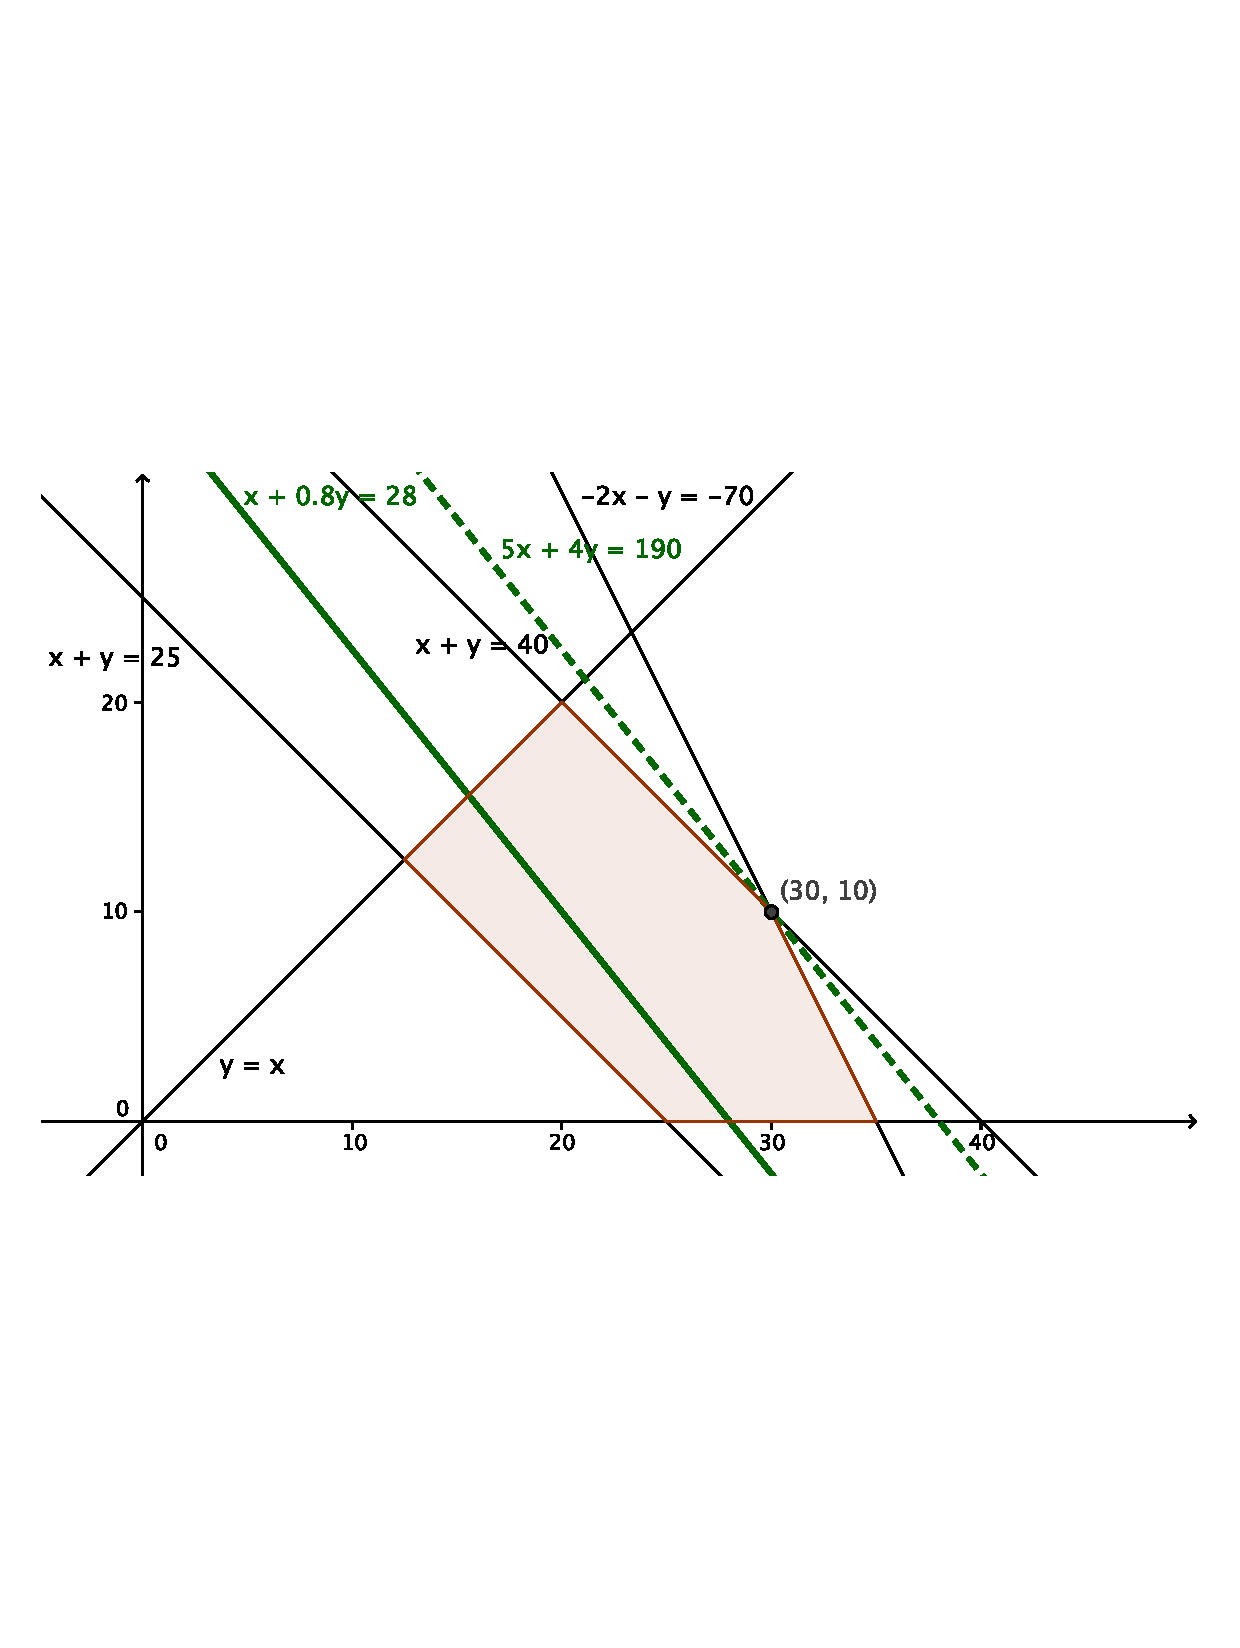
\includegraphics[width=0.8\textwidth]{oefeningen/FigurenLP/Oefpudding.pdf}
\caption{Maximale winst bij 30 potjes vanille- en 10 chocoladepudding}
\label{fig:pudding}
\end{figure}
\end{opl}
\end{oef}

\begin{oef}
Een houthakker kapt in het bos vogelkers en eik. 
De houthakker mag niet zoveel kappen als hij wil. De bosgroep hanteert
daarvoor een puntensysteem. Per ha mag er maar voor maximaal 21 punten
gehakt worden. Een vogelkers is 1 punt waard; een eik 3 punten.
Het bos is 5 ha groot.
Een eik is makkelijker te kappen dan een vogelkers. Als de houthakker per dag maar 
\'e\'en soort zou kappen, zou hij op \'e\'en dag 4 vogelkersen of 6 eiken kappen. 
Hij kan maximaal 10 dagen gaan werken in het bos.
Per eik mag de houthakker hoogstens 3 vogelkersen vellen.
Het aantal vogelkers moet minstens \'e\'en derde van het totaal aantal bomen
tellen.
Een eik geeft 10 keer zoveel winst als een vogelkers. Hoeveel bomen van elk soort
moet de houthakker kappen om zo veel mogelijk winst te bekomen? 
\begin{opl}
15 vogelkers, 30 eiken
\end{opl}
\end{oef}

\begin{oef}    
Een bouwbedrijf specialiseerde zich in het verbouwen van oude panden tot stijlvolle lofts en in de bouw van casco 1-slaapkamer appartementen. Het bedrijf heeft jaarlijks een budget van \SI{20000000}{\euro}. Om dit bedrag te kunnen lenen bij de bank moeten ze garanderen om minstens 10 appartementen en 50 lofts te realiseren. De bouw van een loft kost \SI{200000}{\euro}, een appartement is een stuk goedkoper, dit kost het bedrijf slechts \SI{100000}{\euro}. Het bouwbedrijf werkt nauw samen met een grote algemene aannemer. Deze aannemer kan maximaal personeel leveren voor de bouw van 60 lofts of 135 appartementen. De lofts kunnen anno 2013 verkocht worden aan \SI{300000}{\euro}. Voor een appartementje kan het bedrijf rekenen op een verkoopprijs van \SI{160000}{\euro}. Hoeveel lofts en appartementen moet het bedrijf realiseren en verkopen om zijn winst te maximaliseren?
\begin{opl}
50 lofts en 22 appartementen (eigenlijk 22,5 appartementen, maar je kan geen half appartement bouwen)
\begin{figure}[htb]
\centering
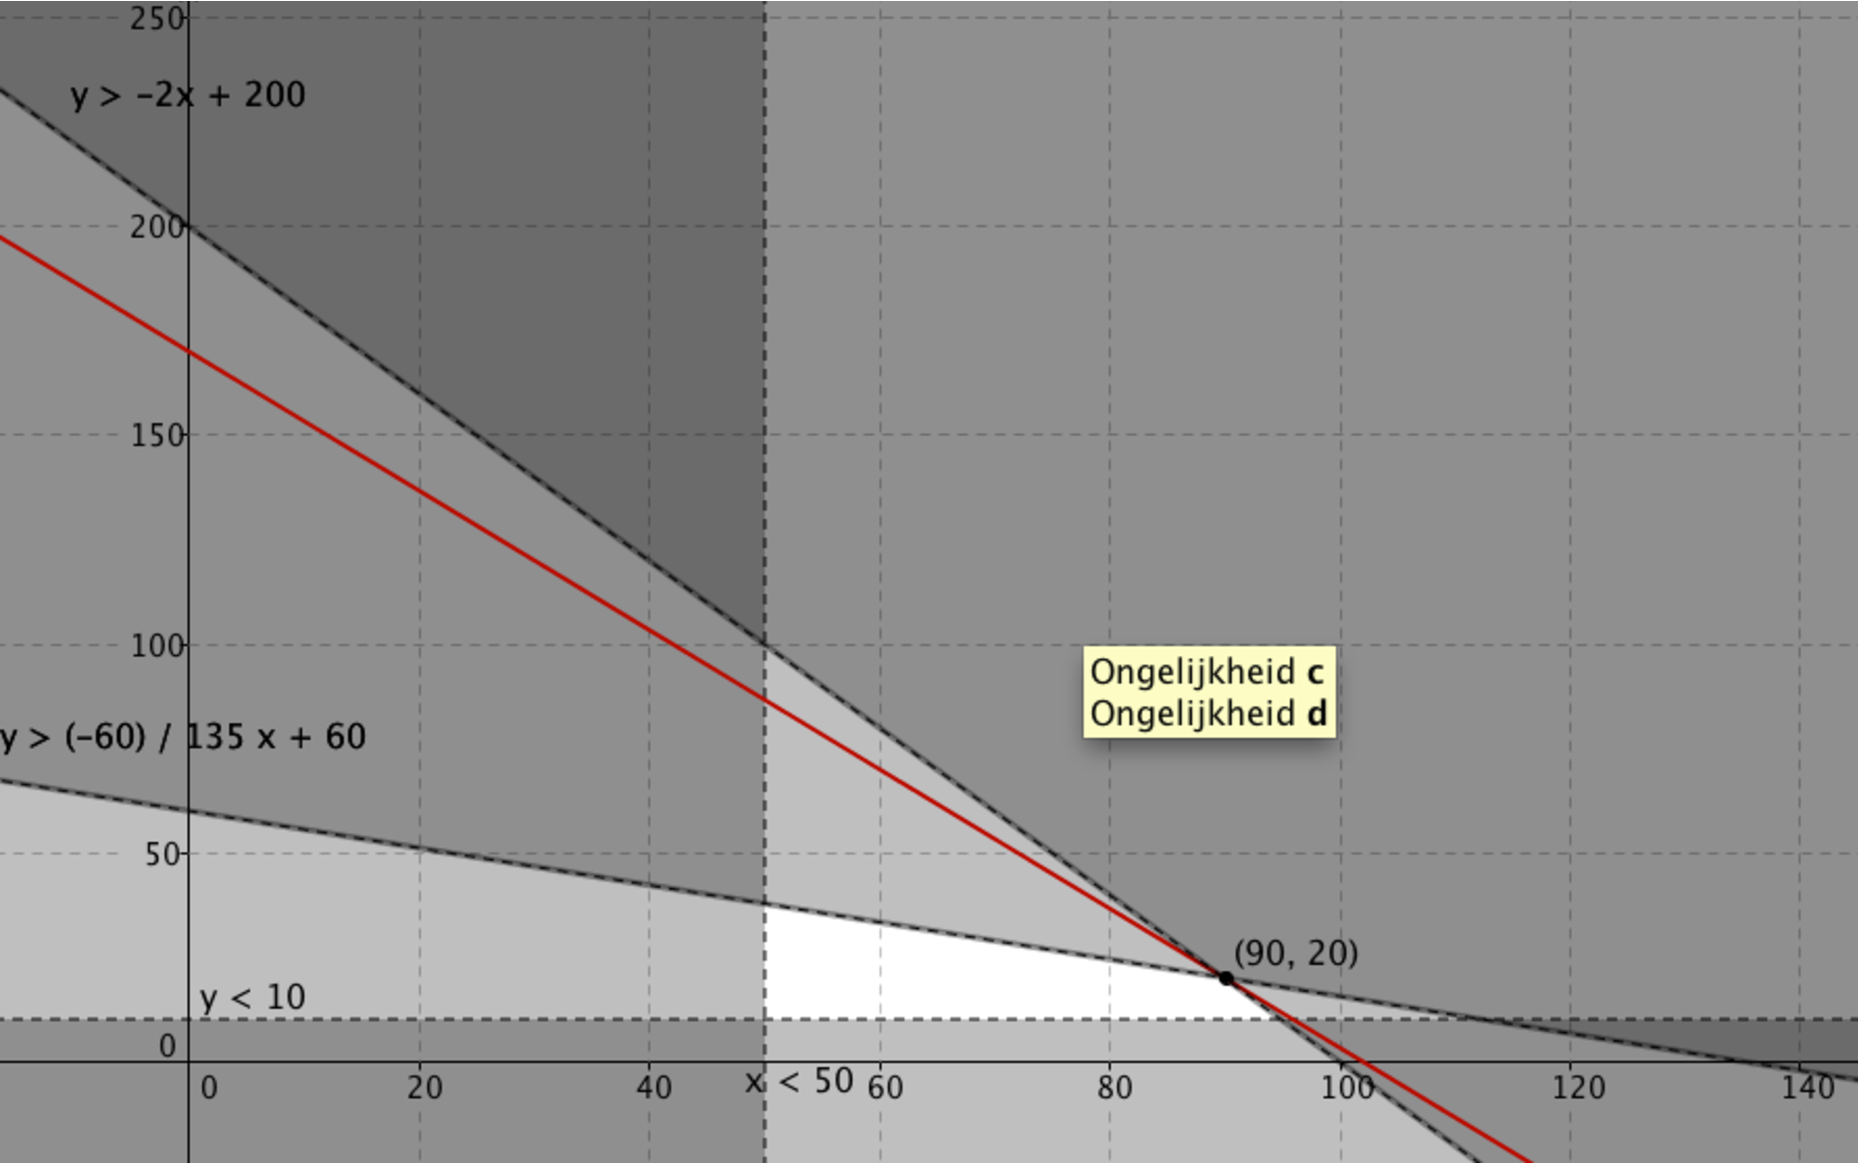
\includegraphics[width=0.8\textwidth]{oefeningen/FigurenLP/lofts}
\end{figure}
\end{opl}
\end{oef}



%\end{document}


%%% Local Variables: 
%%% mode: latex
%%% TeX-master: "cursusTW1"
%%% End: 
